\begin{figure*}[!t]
 \centering
 \subfloat[Varying $\epsilon_{sp}$]{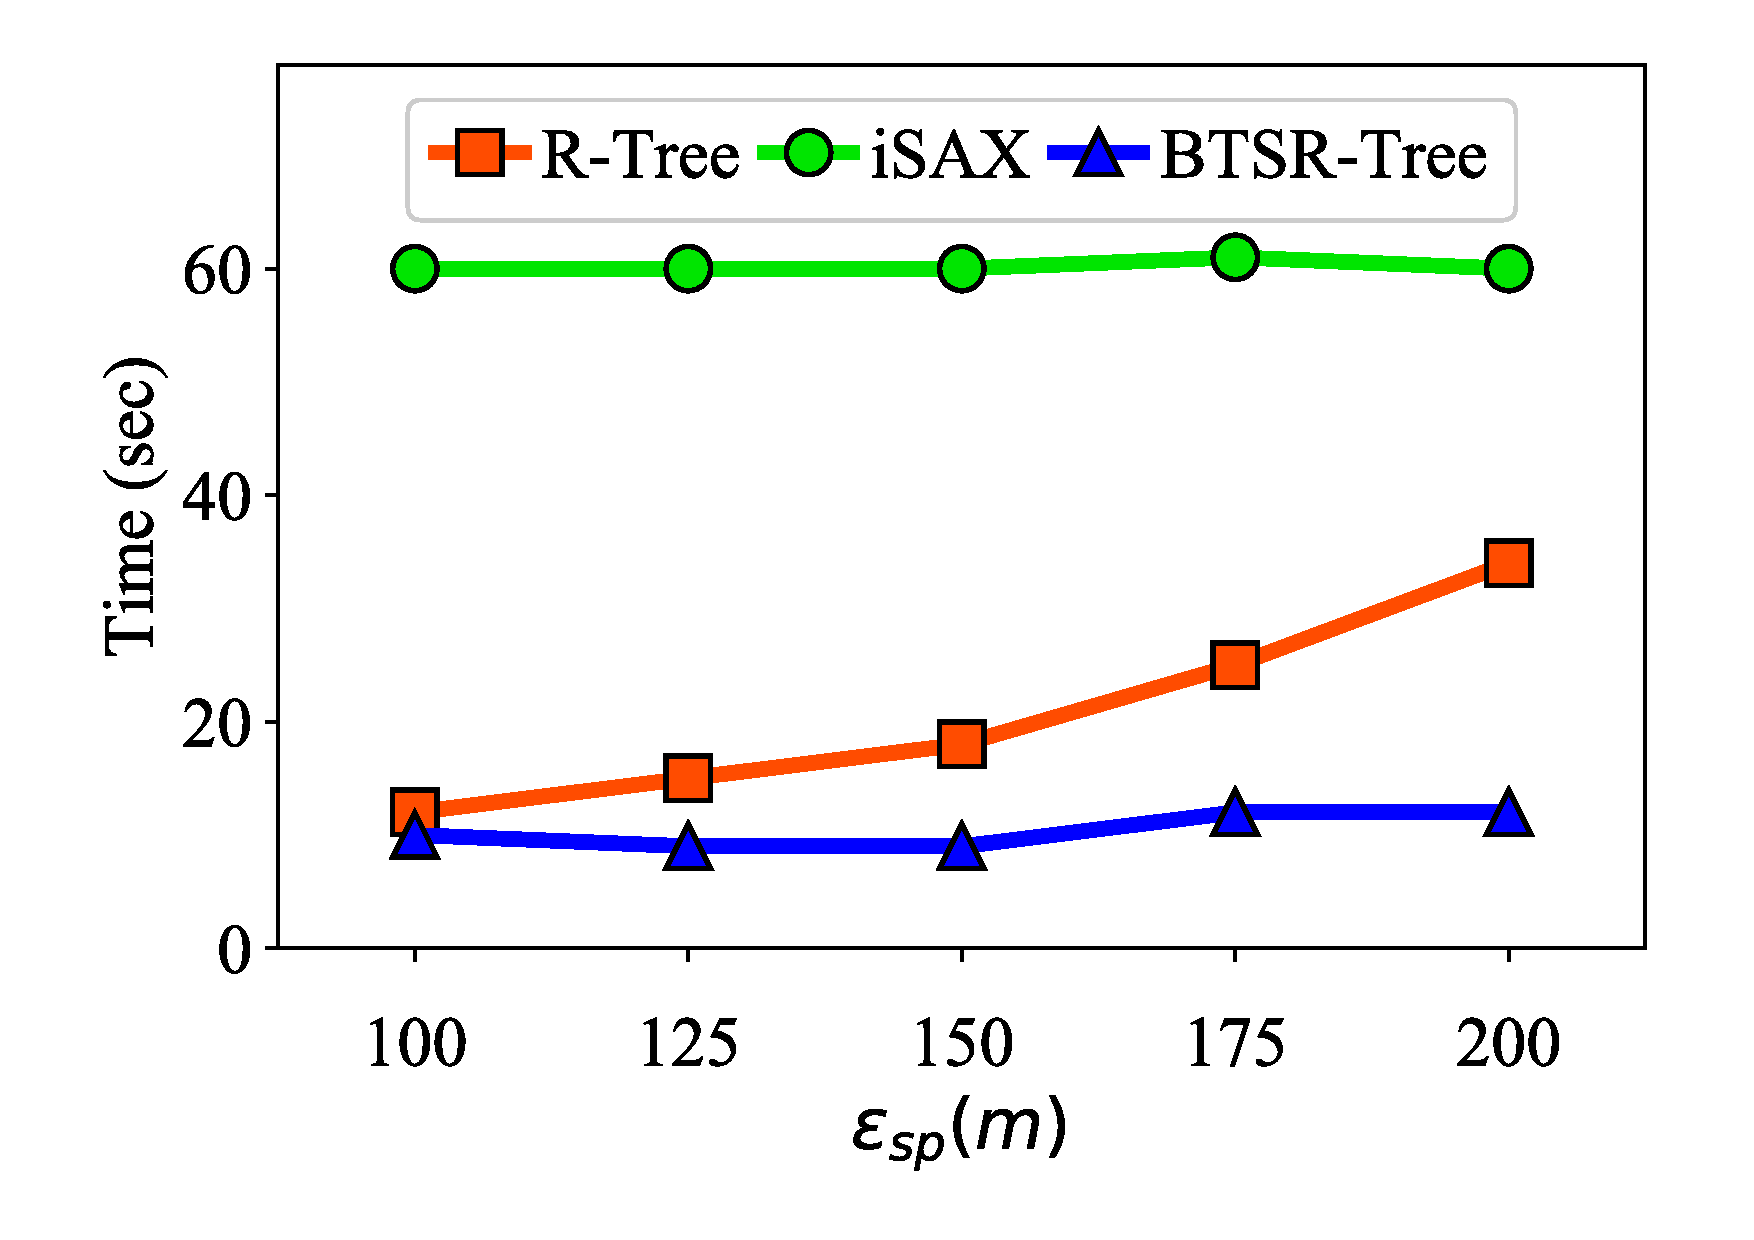
\includegraphics[trim=0.5cm 0.5cm 1cm 1cm, clip, width=0.32\textwidth]{figures/plots/EpsSPCentralized.pdf}\label{exp:EpsSPCentralized}}
 \subfloat[Varying $\epsilon_{ts}$]{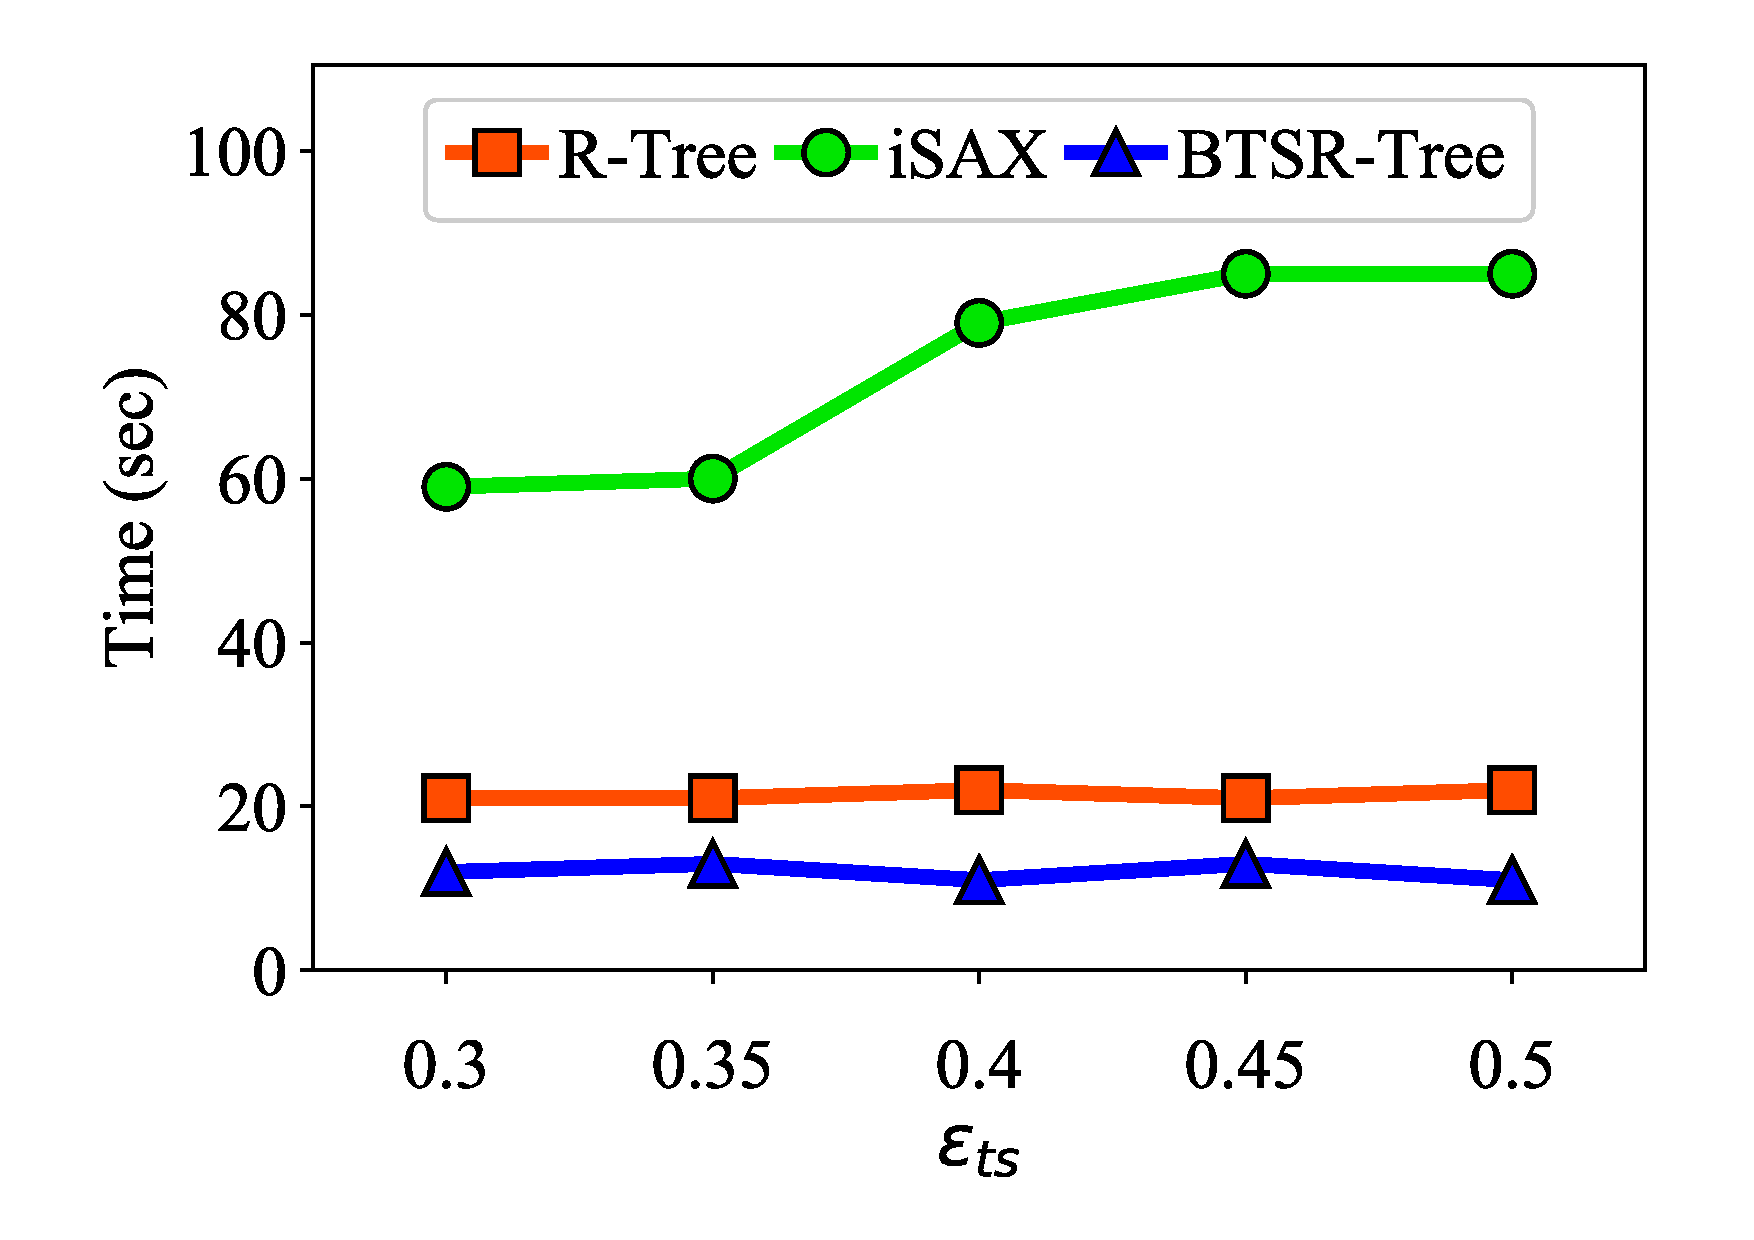
\includegraphics[trim=0.5cm 0.5cm 1cm 1cm, clip, width=0.32\textwidth]{figures/plots/EpsTSCentralized.pdf}\label{exp:EpsTSCentralized}}
 \subfloat[Scalability]{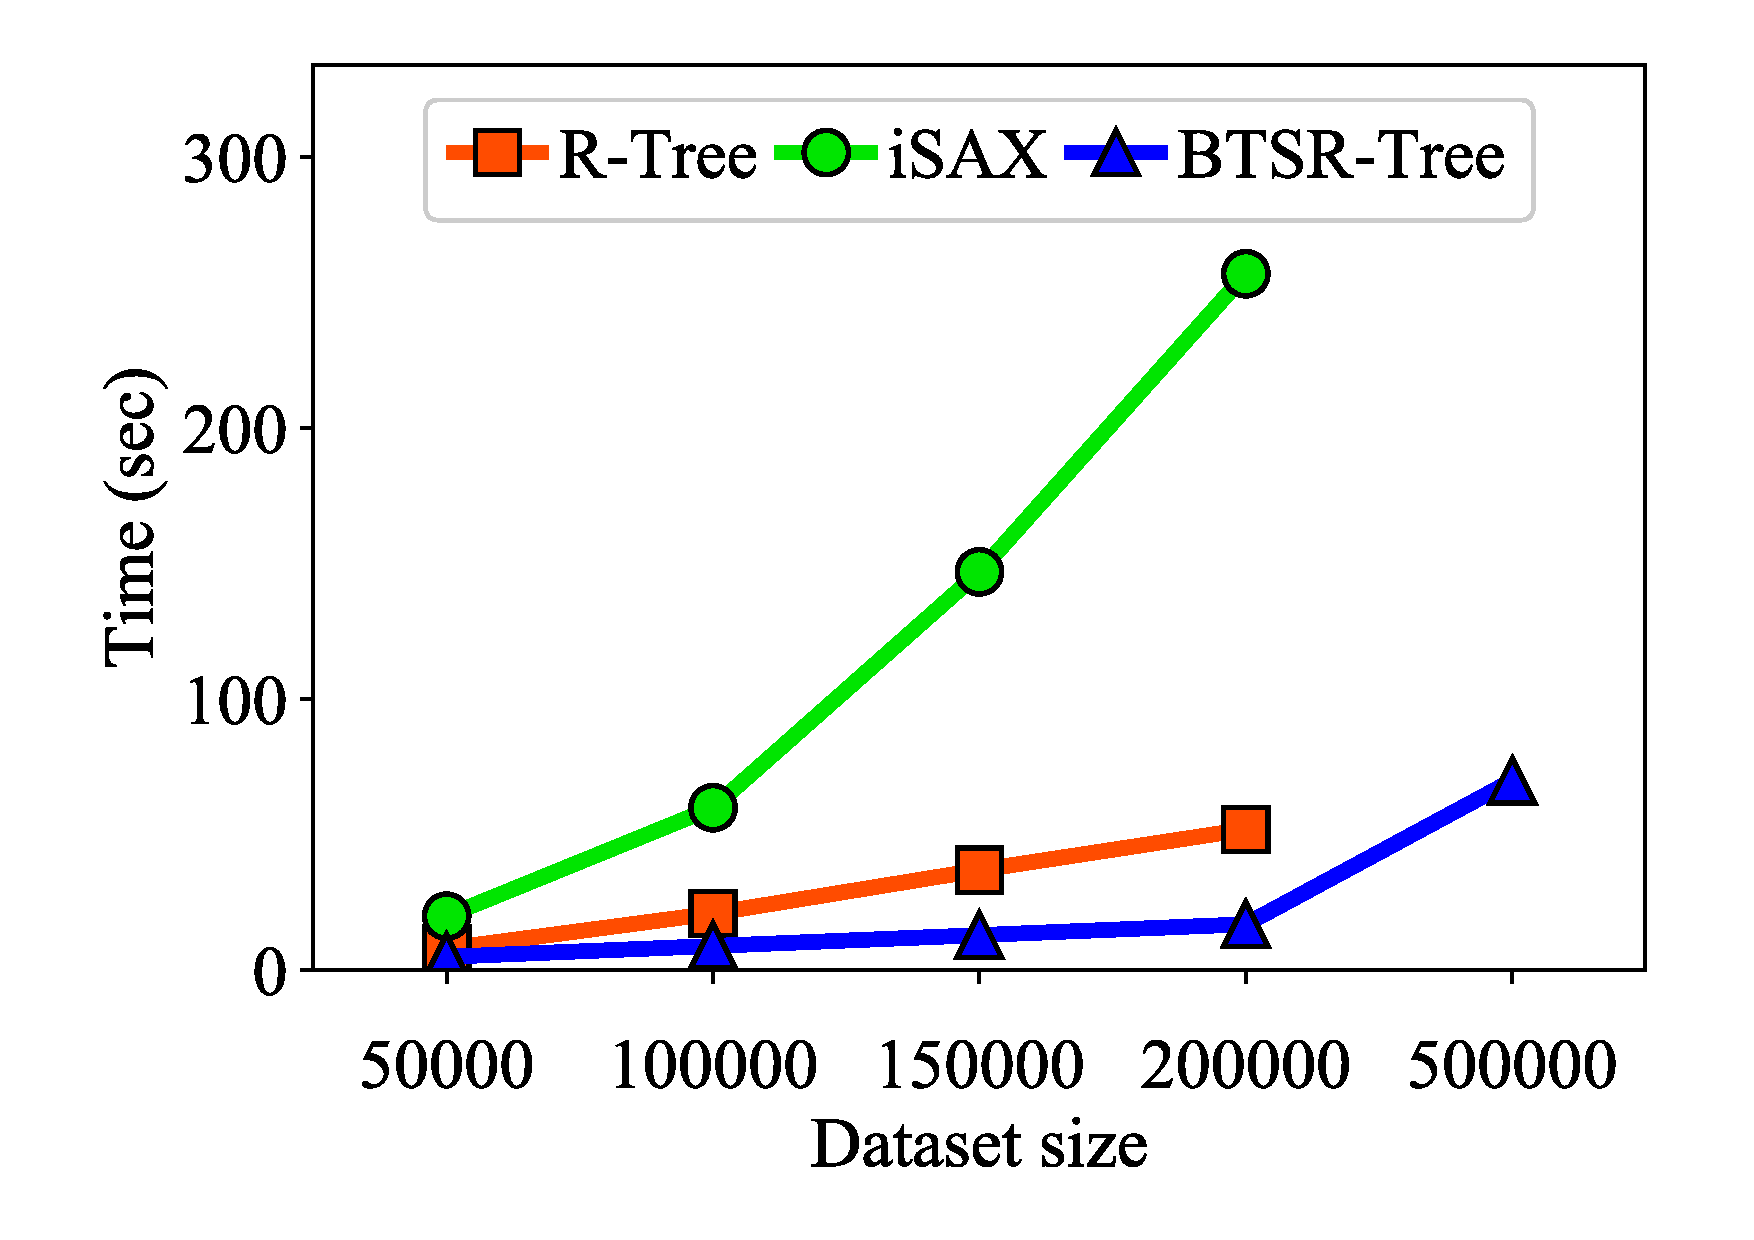
\includegraphics[trim=0.5cm 0.5cm 1cm 1cm, clip, width=0.32\textwidth]{figures/plots/ScalabilityCentralized.pdf}\label{exp:ScalabilityCentralized}}
 \caption{Processing cost for {\em centralized} execution of similarity join queries employing different indices.}
 \label{exp:centralized}
\end{figure*}



\vspace{-2mm}
\subsection{Experimental Evaluation}
\label{sec:evaluation}

%Next, we first describe our experimental setup, and then we report results from an extensive evaluation of the proposed algorithms.

\subsubsection{Experimental Setup}
\label{subsec:evaluation_setup}

%\subsubsection{Datasets}
%\label{subsubsec:datasets}

We generated several {\em synthetic} datasets of various sizes, using a real-world water consumption dataset as a seed. This real dataset, provided by the DAIAD project (\url{http://daiad.eu/}), contained geolocated time series of hourly water consumption for 822 households in Alicante, Spain from 1/1/2015 to 20/1/2017. On this data, we first calculated the weekly  ($24 \times 7$) time series per household by averaging corresponding hourly values over the entire period. Then, these weekly sequences were used as seeds to synthetically increase the size of the dataset up to 2 million geolocated time series, by introducing small random variations in their location and pattern.

%\footnote{\url{http://daiad.eu/}}

%\subsubsection{Evaluation Parameters}
%\label{subsubsec:parameters}

In preliminary tests, we fine-tuned parameters for the various indices used against this data. For {\btsr}s and {\rtree}s, the number of entries per node ranges between $m$=10 and $M$=50. 
In \isax, up to $M$=250 time series can be stored per leaf and the length of each SAX word is $w$=8. Table~\ref{tab:parameters} lists the range of values for the rest of parameters used in our tests; default values are in bold. 




\begin{table}[t]
\centering
\caption{Parameters tested in the experiments}
 \vspace{-10pt}
\begin{footnotesize}
\begin{tabular}{lc} 
\hline
{\em Parameter} &{\em Values} \\
\hline
%\hline{}
Dataset size ({\em centralized}) & 50K, 100K, 150K, {\bf 200K}, 500K, 1000K \\
%\hline
Dataset size ({\em distributed}) & 500K, {\bf 1000K}, 1500K, 2000K \\
%\hline
Number of partitions $g\times g$ ({\em distributed}) & $10^2$, $20^2$, ${\bf 30^2}$,$40^2$,$50^2$,$60^2$,$70^2$ \\
%\hline
Distance radius $\epsilon_{sp}$ (meters) in queries & 100, 125, {\bf 150}, 175, 200 \\
%\hline
Time series deviation $\epsilon_{ts}$ in queries & 0.3, {\bf 0.35}, 0.4, 0.45, 0.5 \\
\hline
\end{tabular}
\end{footnotesize}
\label{tab:parameters}
\end{table}



%Regarding the evaluation parameters, we have selected the default $\epsilon_{sp}$ to be 150 meters, the $\epsilon_{ts}$ to 0.35, the default dataset size to 1,000,000 and the default partitioning level to $30 \times 30$.

%\subsubsection{Evaluation Setting}
%\label{subsubsec:setting}



\begin{figure*}[!t]
 \centering
 \subfloat[Query response time]{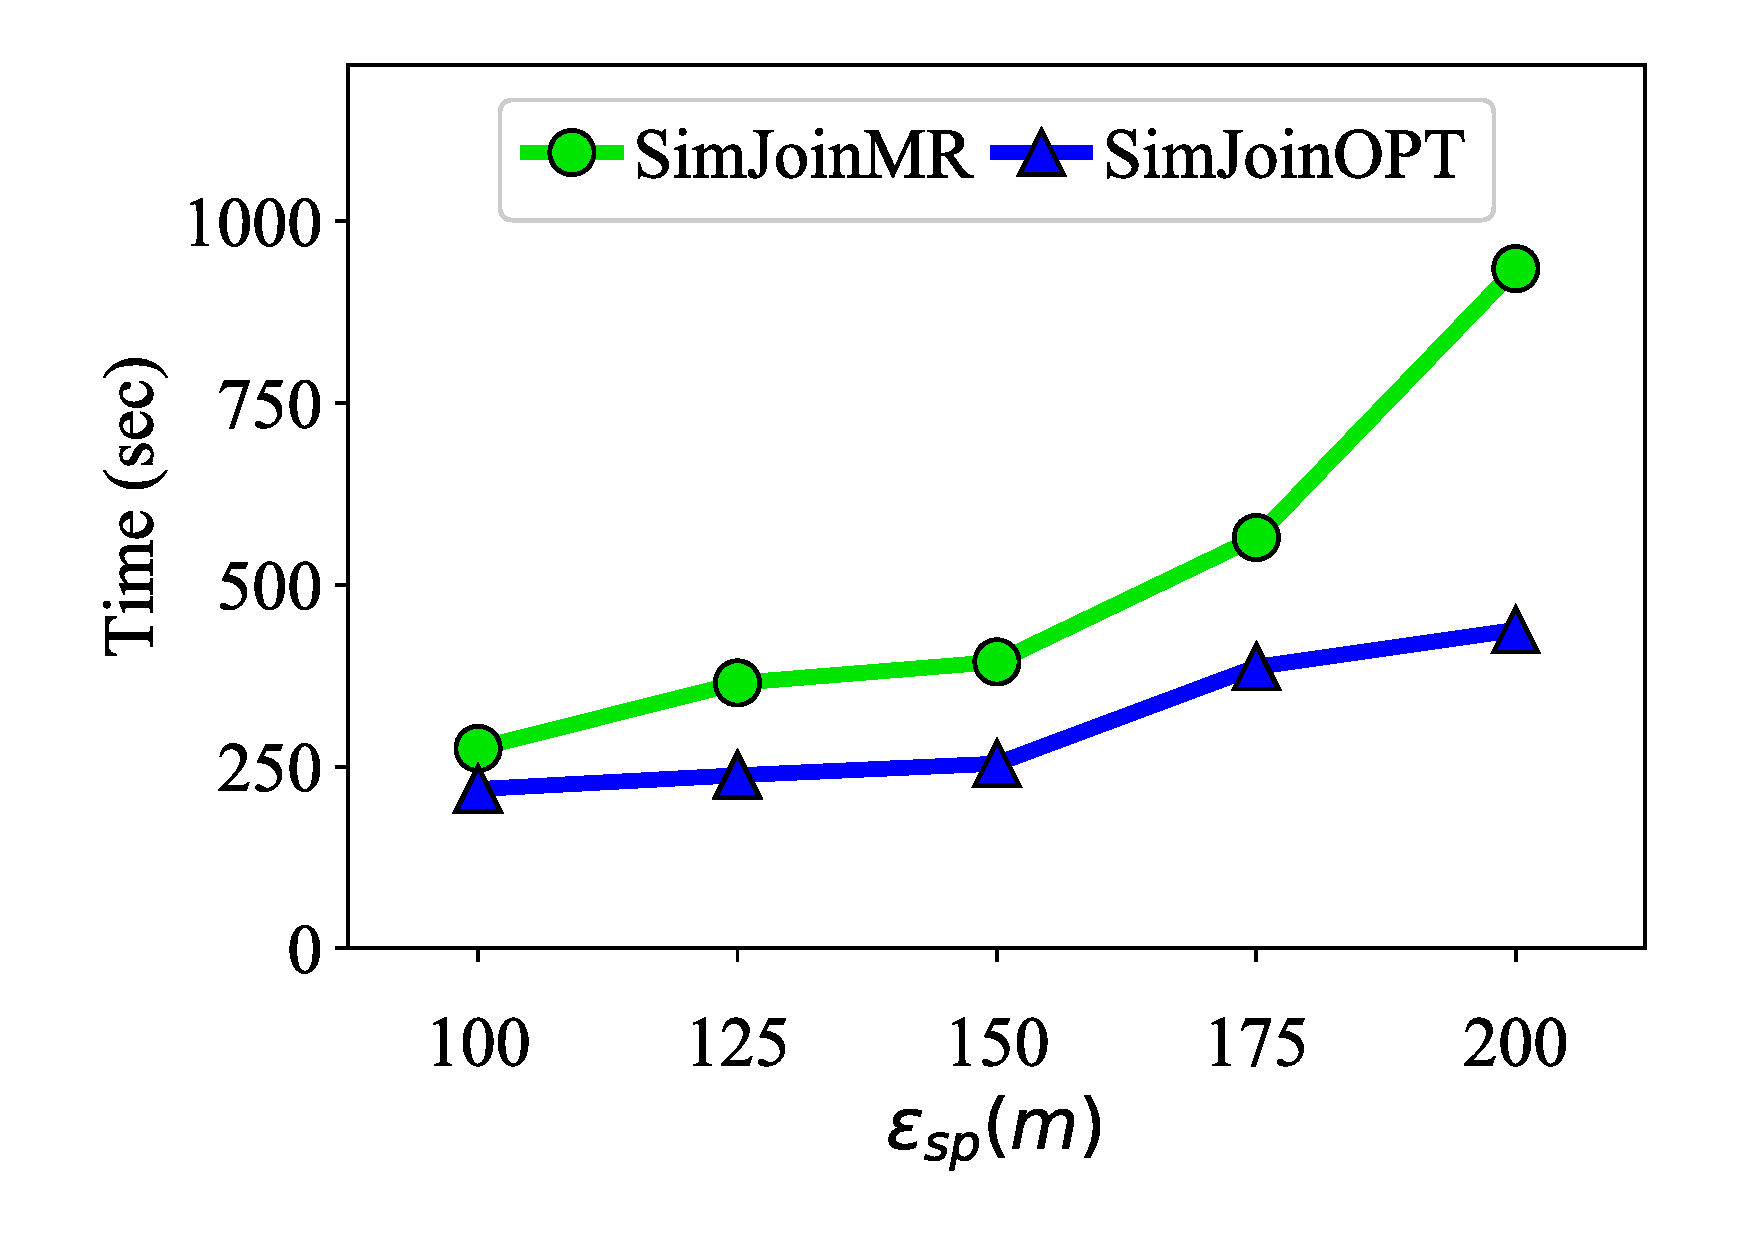
\includegraphics[trim=0.5cm 0.5cm 1cm 1cm, clip, width=0.32\textwidth]{figures/plots/EpsSPDist.pdf}\label{exp:EpsSPDist}}
 \subfloat[Geolocated time series shuffled]{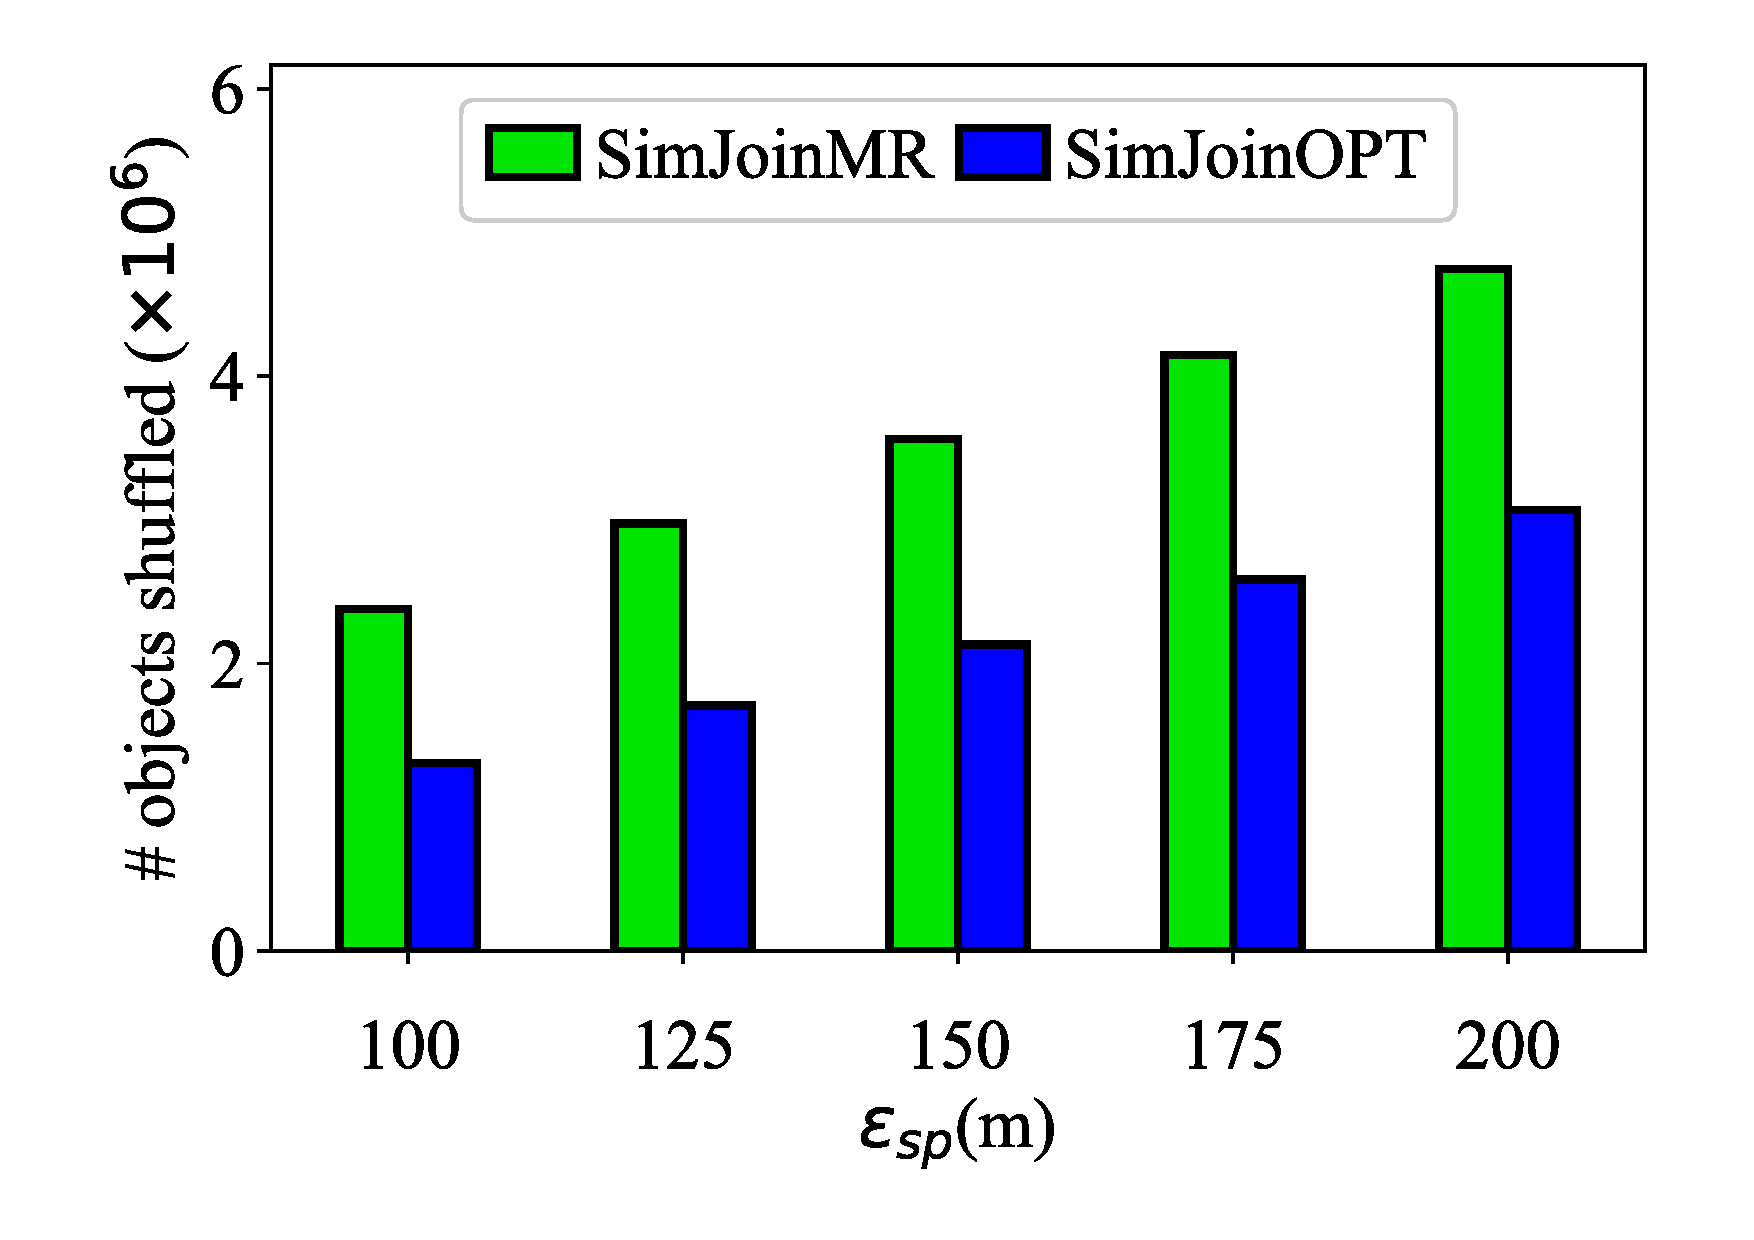
\includegraphics[trim=0.5cm 0.5cm 1cm 1cm, clip, width=0.32\textwidth]{figures/plots/EpsSPDistCommunication.pdf}\label{exp:EpsSPDistCommunication}}
 \subfloat[Number of query results per phase]{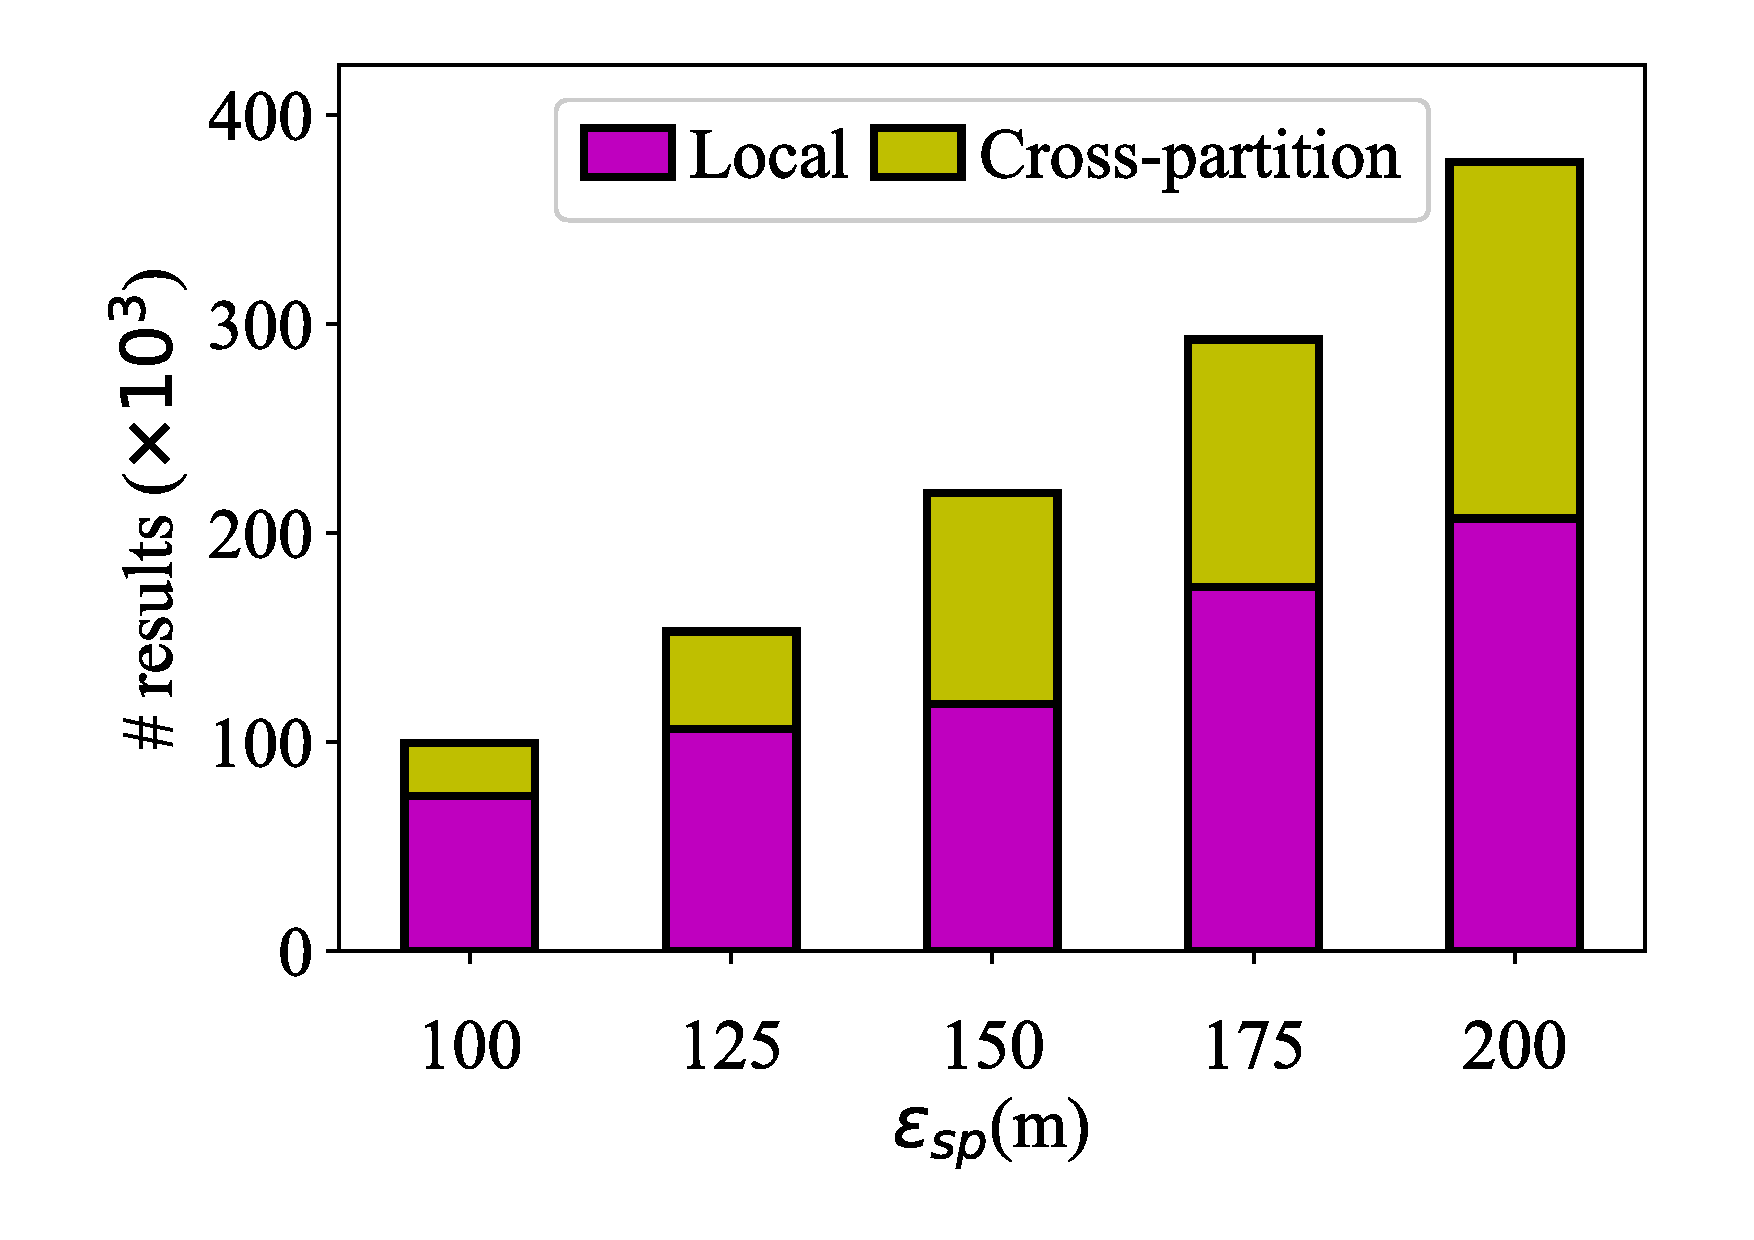
\includegraphics[trim=0.3cm 0.5cm 1.2cm 1cm, clip, width=0.32\textwidth]{figures/plots/EpsSPDistResults.pdf}\label{exp:EpsSPDistResults}}
 \caption{Performance results for the {\em distributed} methods with varying $\epsilon_{sp}$.}
 \label{exp:distr_EpsSP}
\end{figure*}





All algorithms were implemented in Java. Distributed methods were developed on Apache Spark 2.3.0. The centralized experiments were executed on a machine running MacOS 10.13.5 with a 2GHz CPU and 8GB of RAM. The distributed tests were conducted on a cluster with 7 virtual machines running Ubuntu 16.04.3 LTS, with 4 cores each, clocked at 2100MHz. Each node had a total of 5GB of RAM. Next, we report performance in terms of average response time per query. Each query runs against two instances of the same dataset (i.e., {\em self-join}), excluding identity matches from resulting pairs. In the distributed case, we also measure the amount of raw data transferred between workers during the cross-partition phase. 


\subsubsection{Evaluation Results}
\label{subsec:exp_results}


\begin{figure*}[!t]
 \centering
 \subfloat[Query response time]{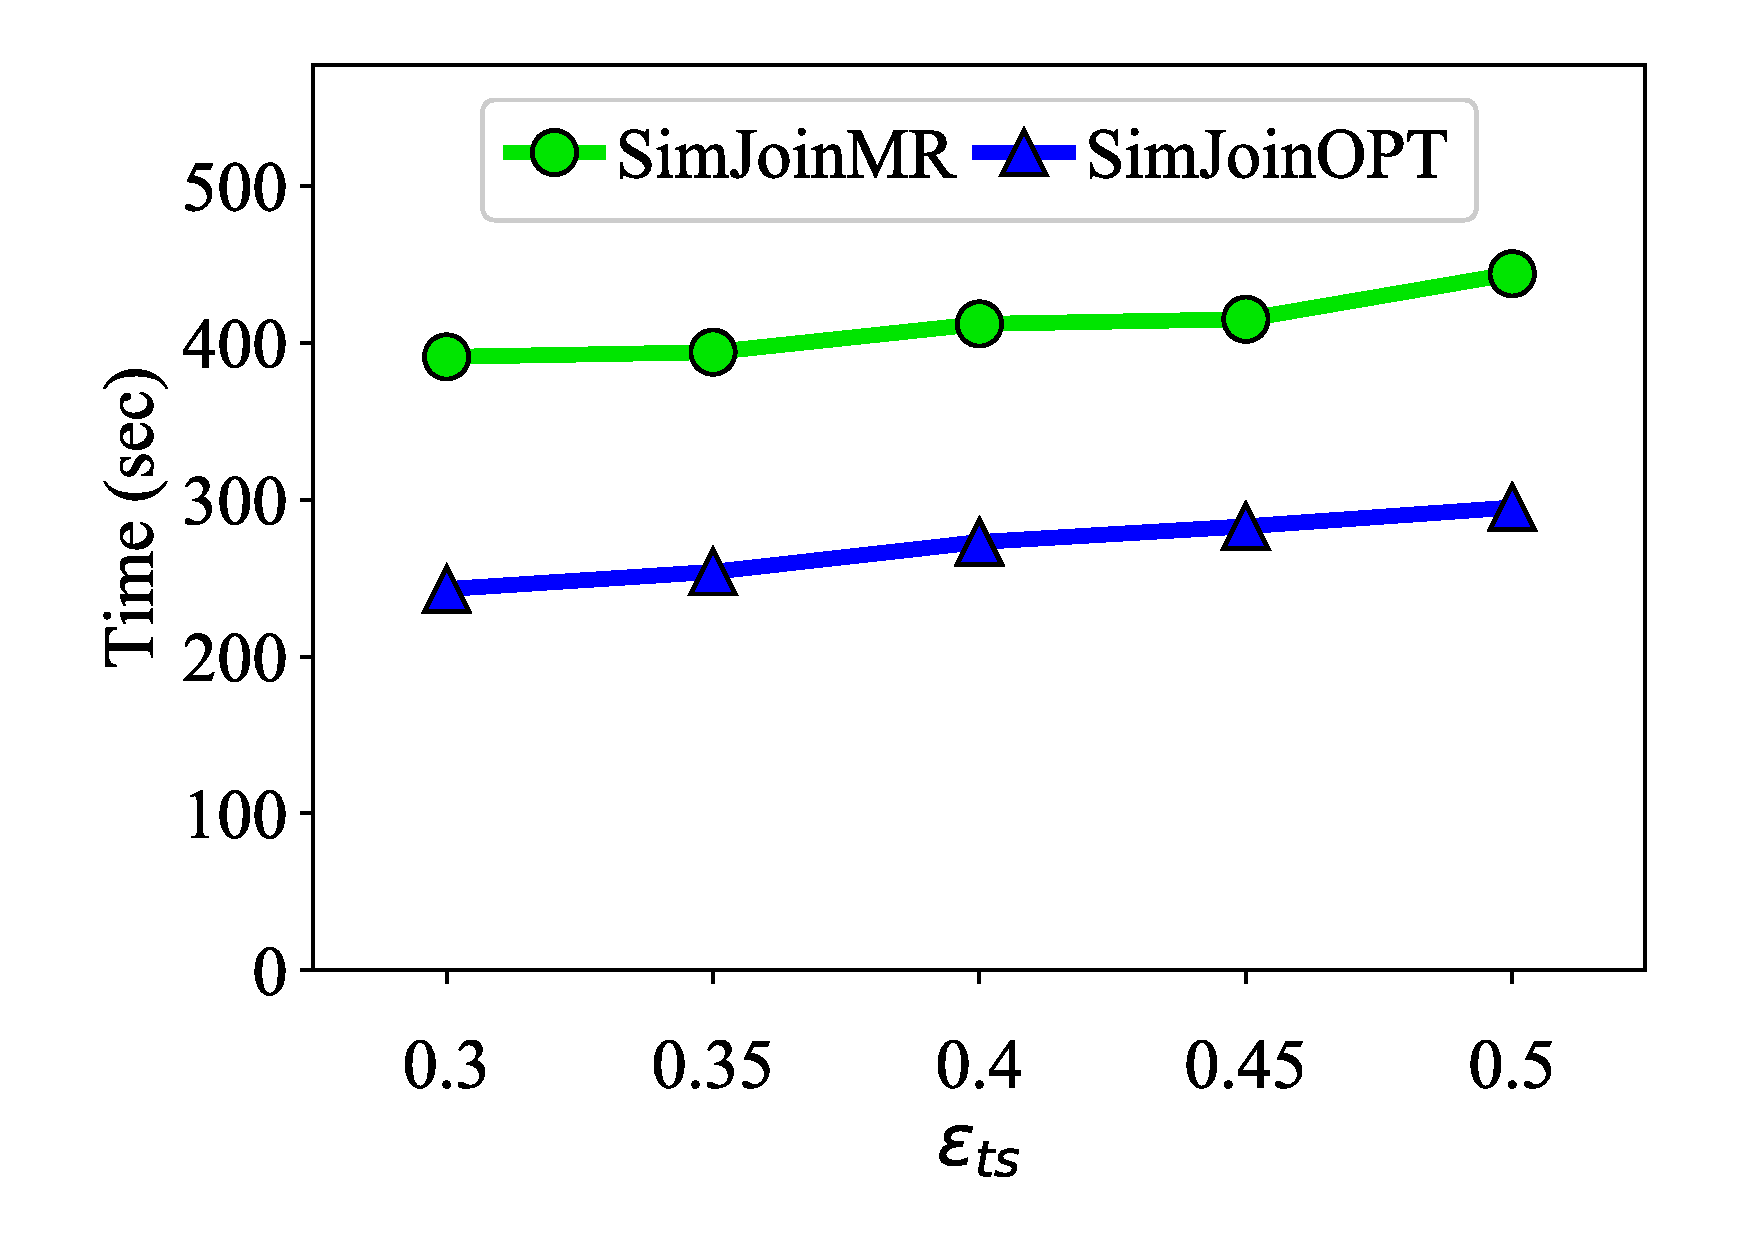
\includegraphics[trim=0.5cm 0.5cm 1cm 1cm, clip, width=0.32\textwidth]{figures/plots/EpsTSDist.pdf}\label{exp:EpsTSDist}}
 \subfloat[Geolocated time series shuffled]
 {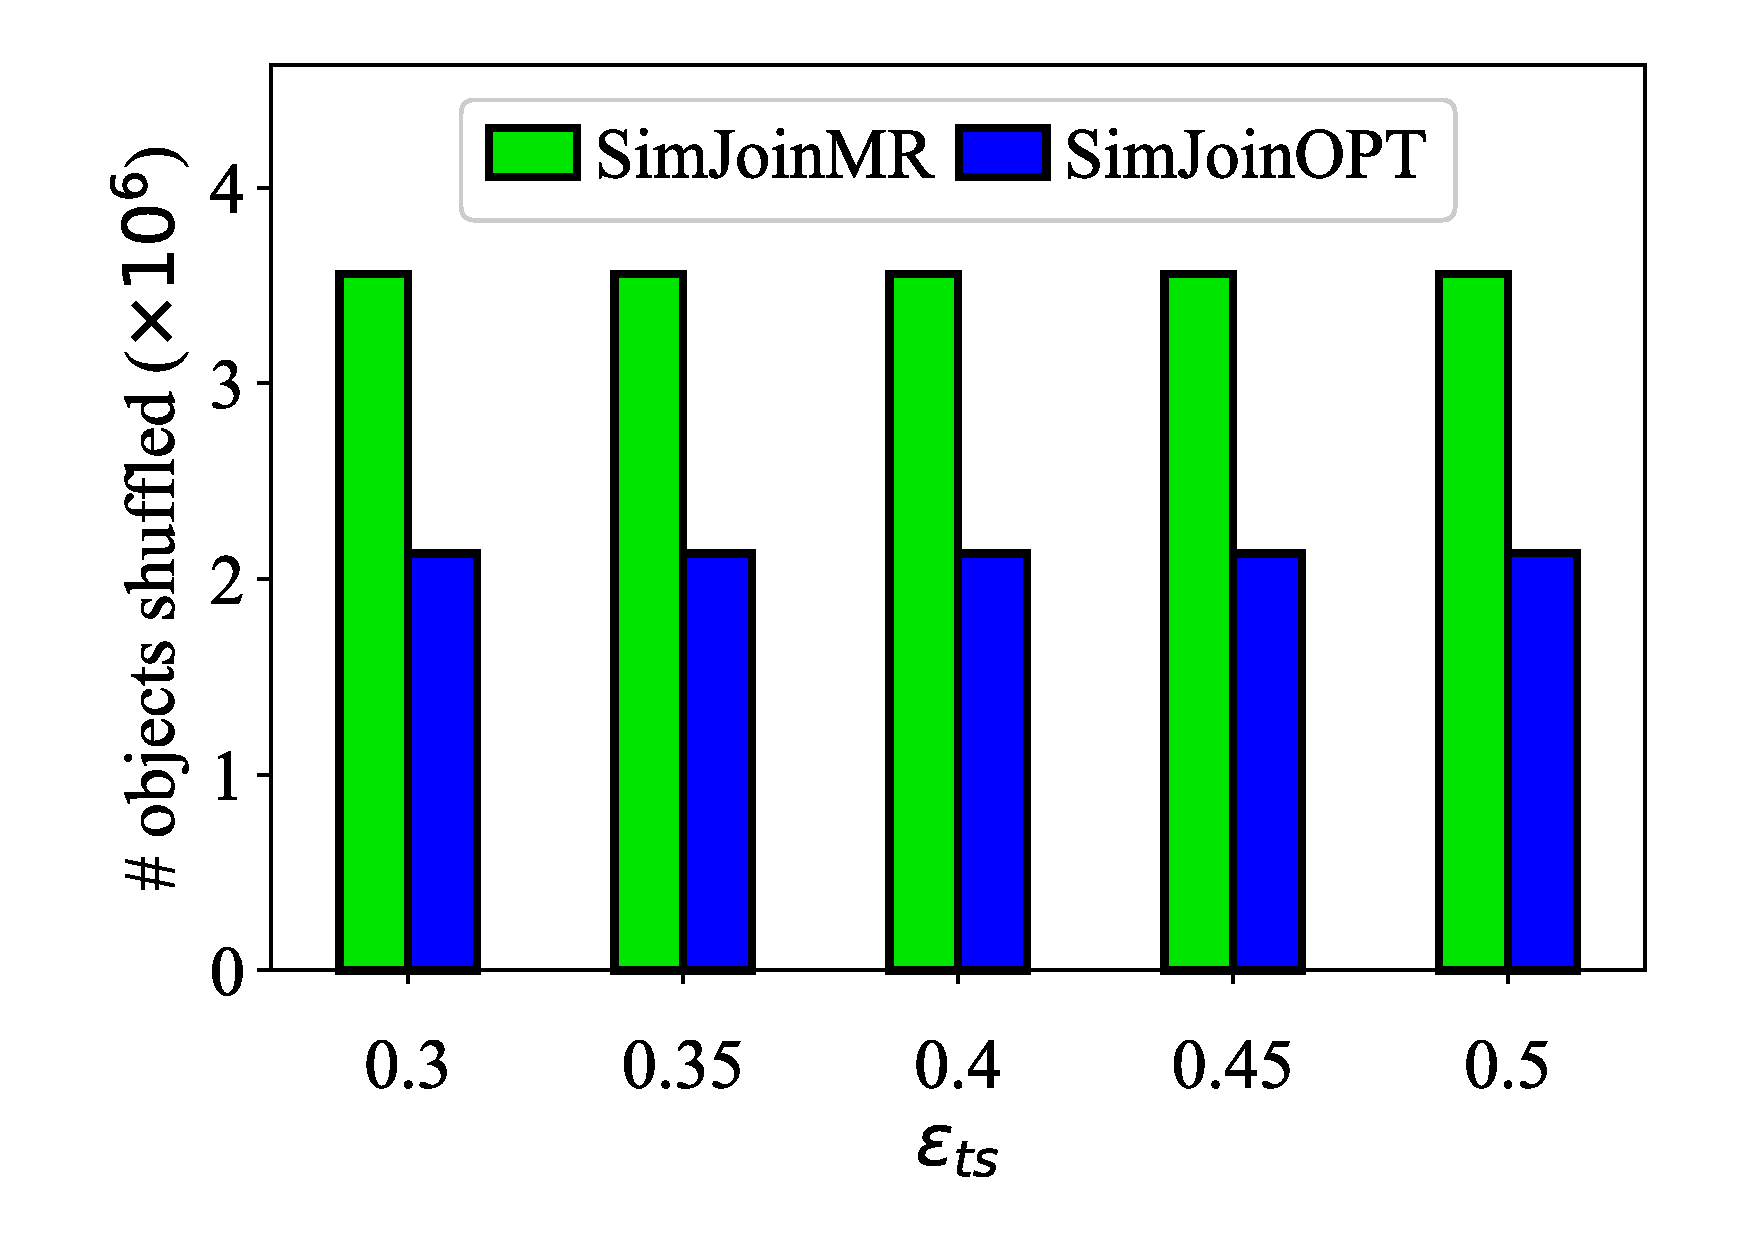
\includegraphics[trim=0.5cm 0.5cm 1cm 1cm, clip, width=0.32\textwidth]{figures/plots/EpsTSDistCommunication.pdf}\label{exp:EpsTSDistCommunication}}
 \subfloat[Number of query results per phase]{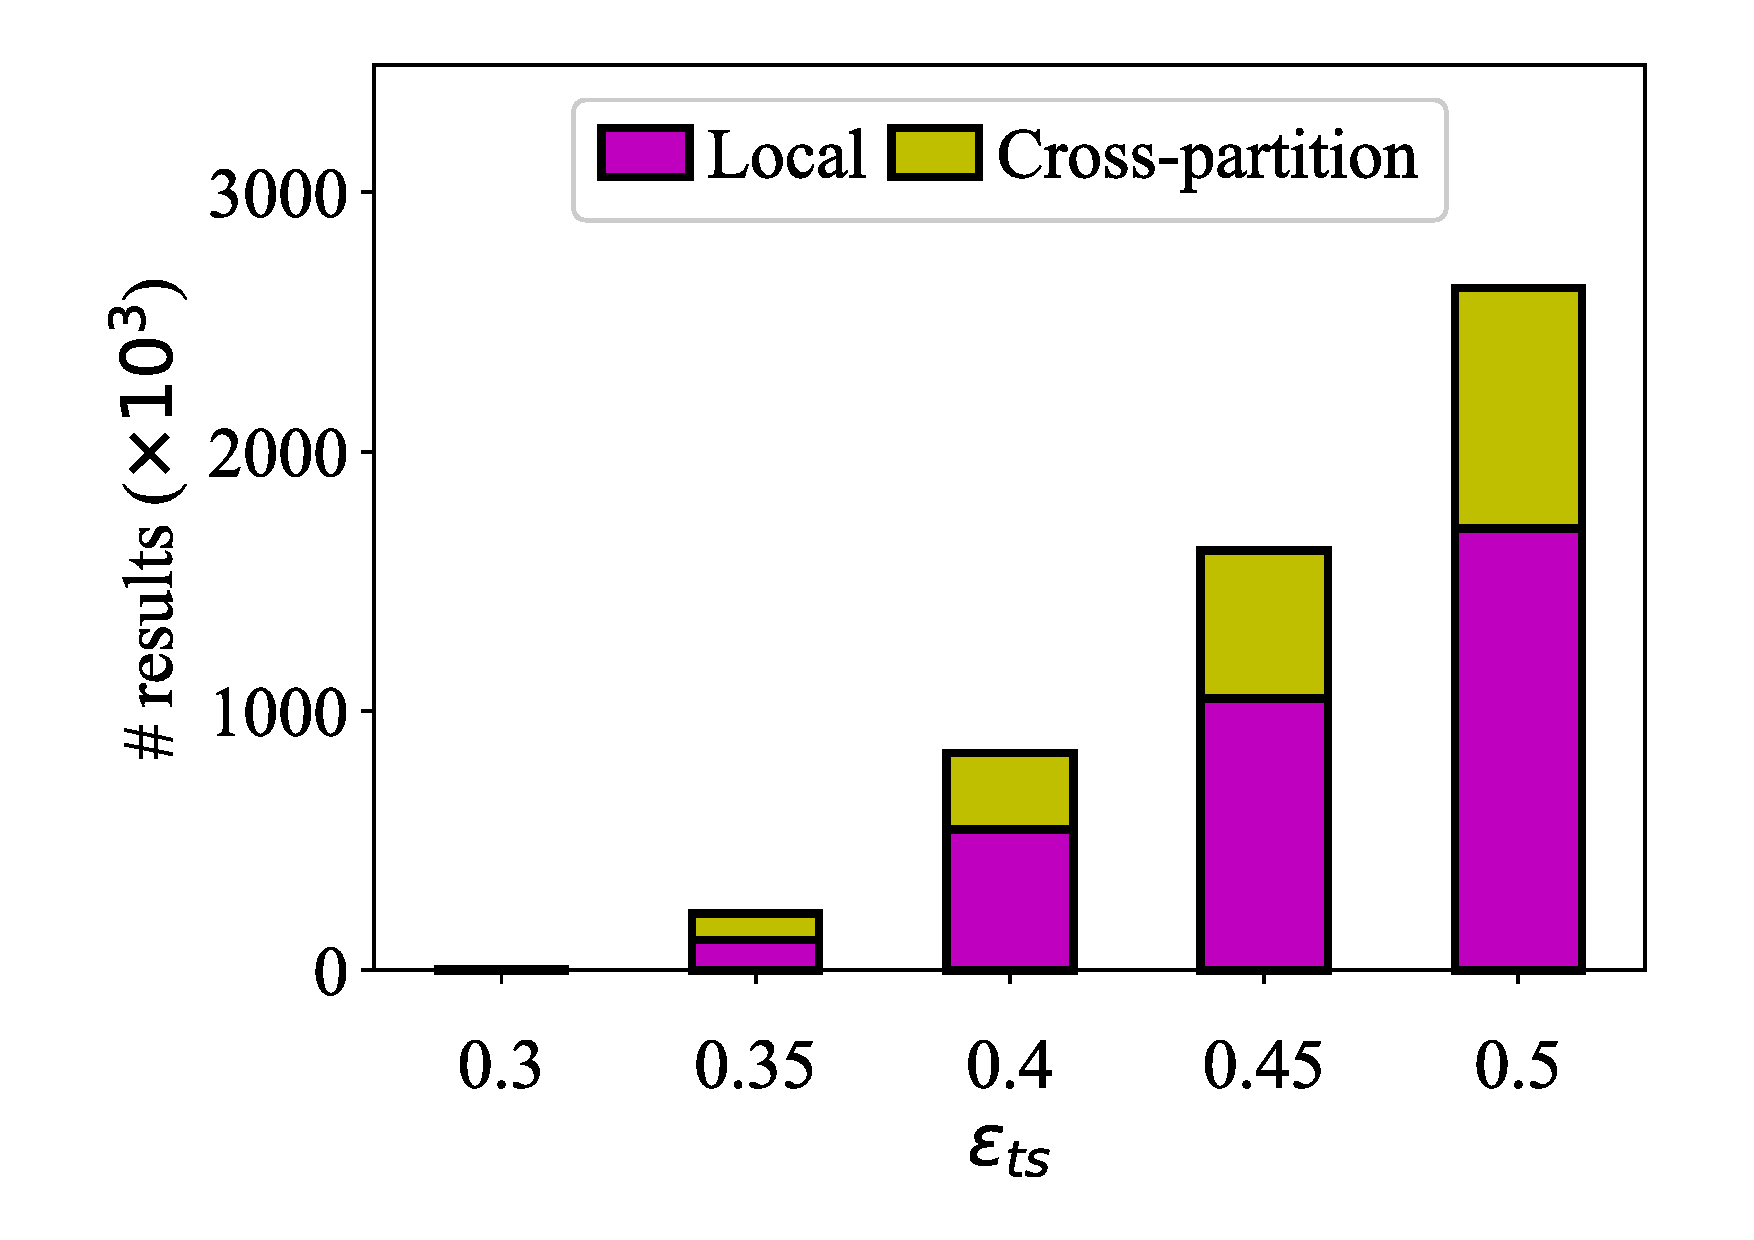
\includegraphics[trim=0 0.5cm 1.4cm 1cm, clip, width=0.32\textwidth]{figures/plots/EpsTSDistResults.pdf}\label{exp:EpsTSDistResults}}
 \caption{Performance results for the {\em distributed} methods with varying $\epsilon_{ts}$.}
 \label{exp:distr_EpsTS}
\end{figure*}

 \begin{figure*}[!t]
 \centering 
 \subfloat[Query response time]{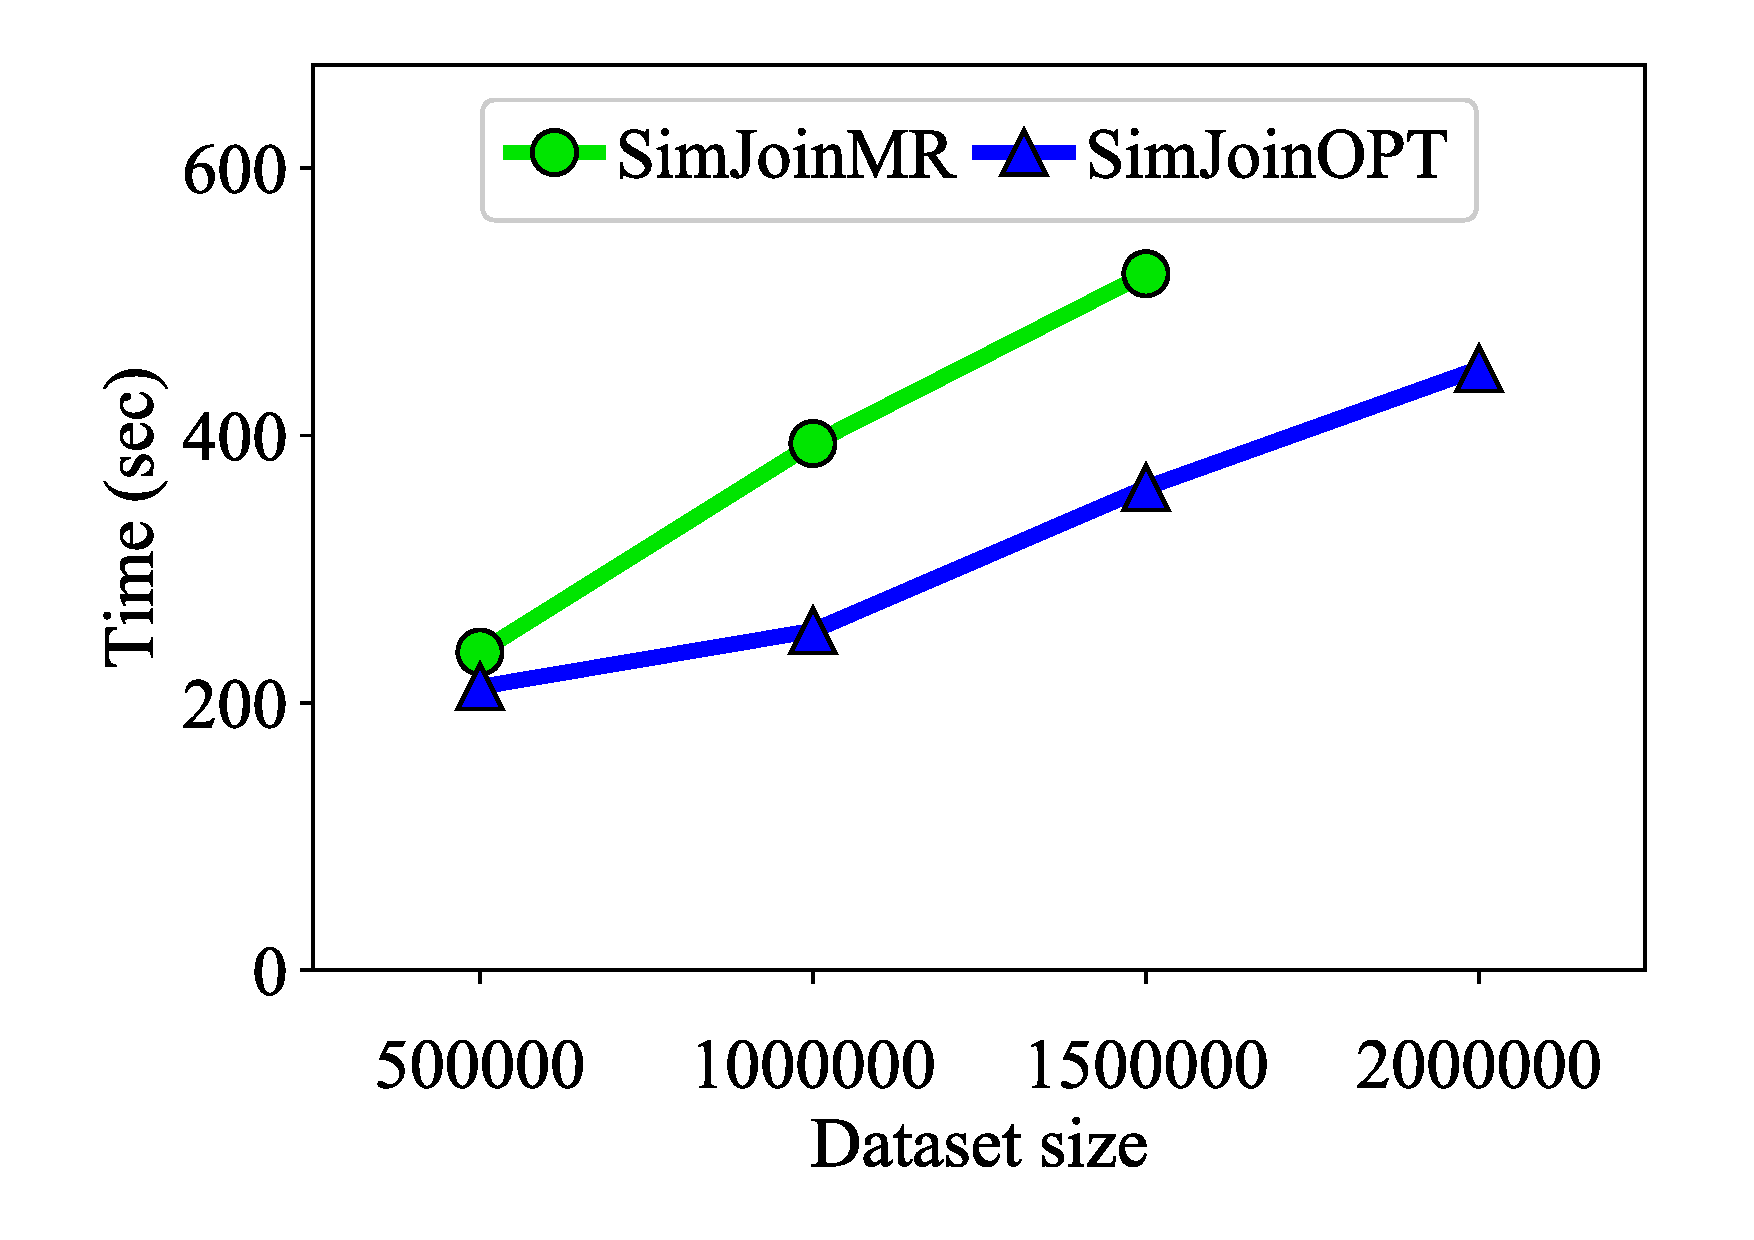
\includegraphics[trim=0.5cm 0.5cm 1cm 1cm, clip, width=0.32\textwidth]{figures/plots/ScalabilityDist.pdf}\label{exp:ScalabilityDist}}
 \subfloat[Geolocated time series shuffled]{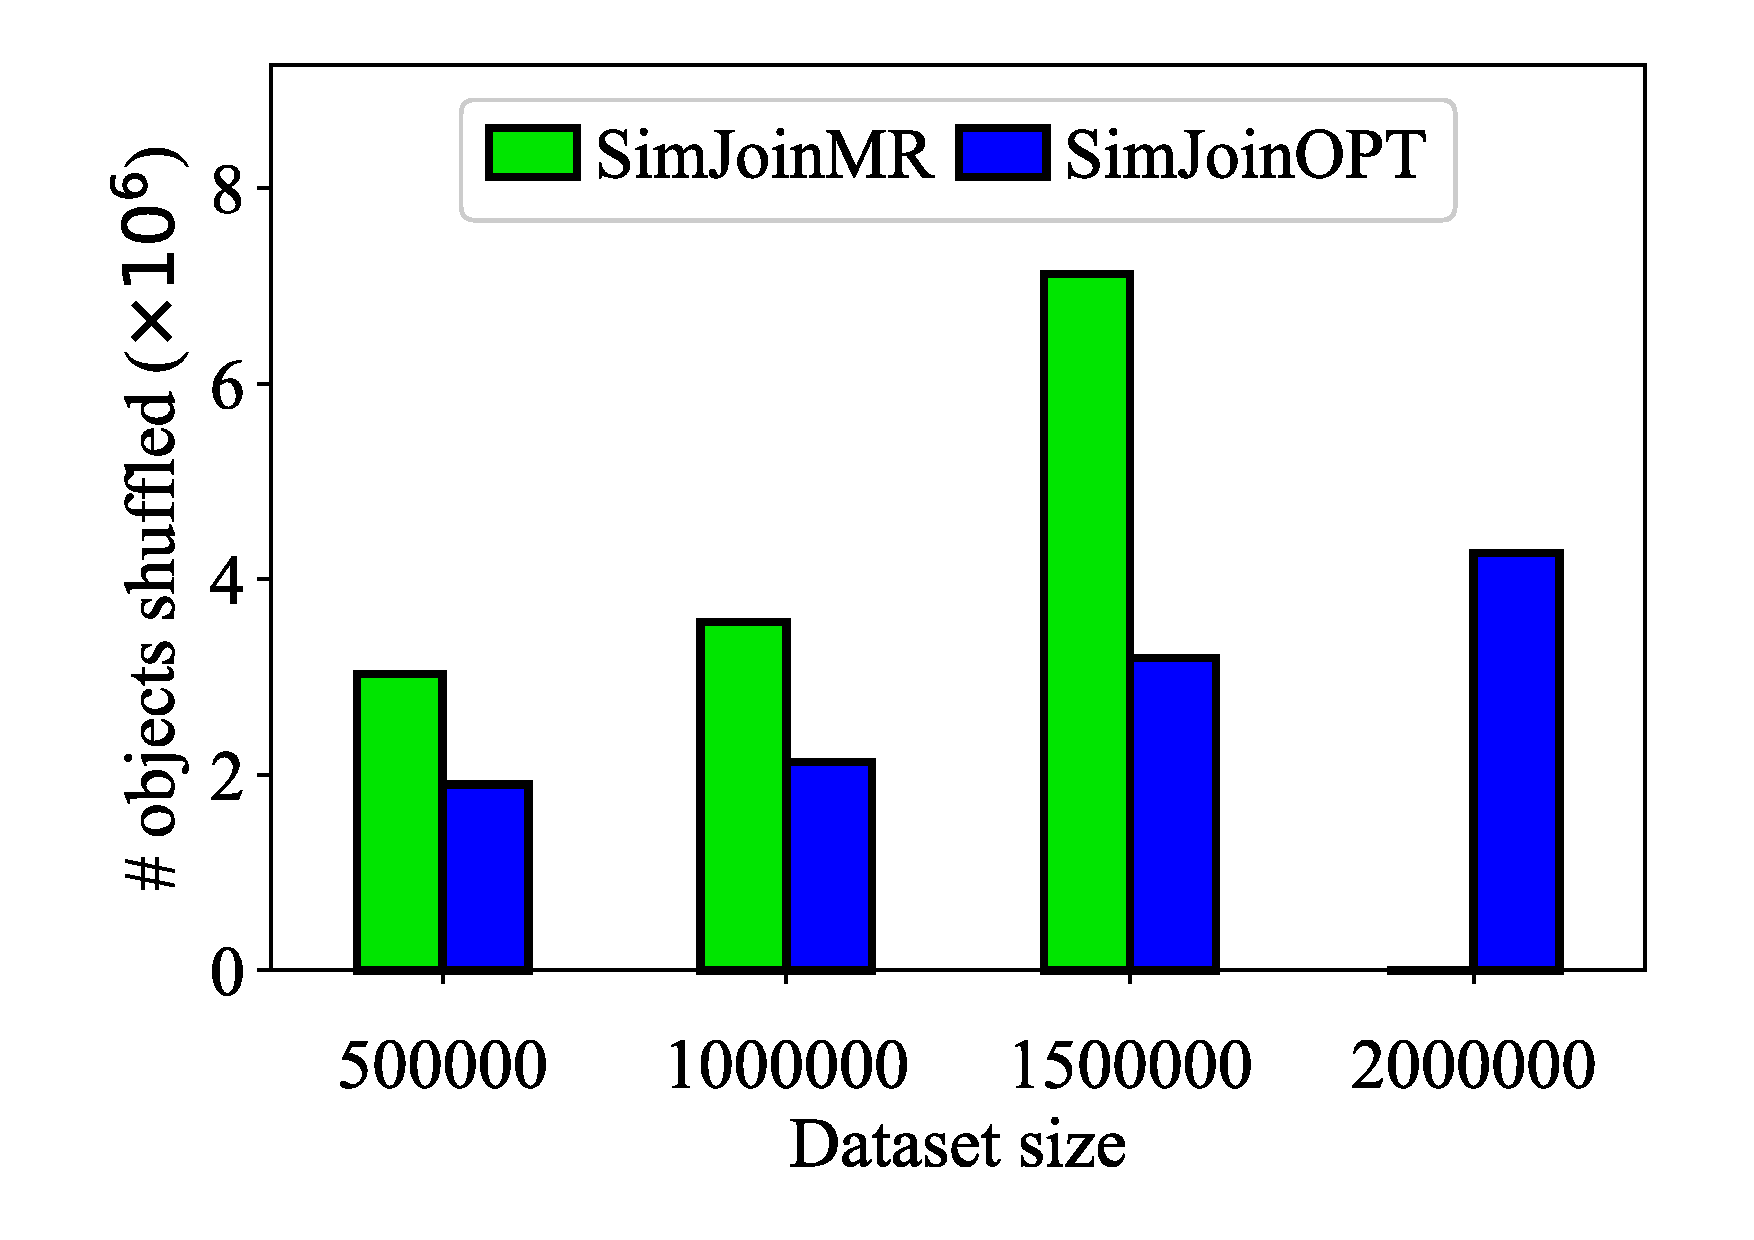
\includegraphics[trim=0.5cm 0.5cm 1cm 1cm, clip, width=0.32\textwidth]{figures/plots/ScalabilityCommunication.pdf}\label{sexp:ScalabilityCommunication}}
 \subfloat[Number of query results per phase]{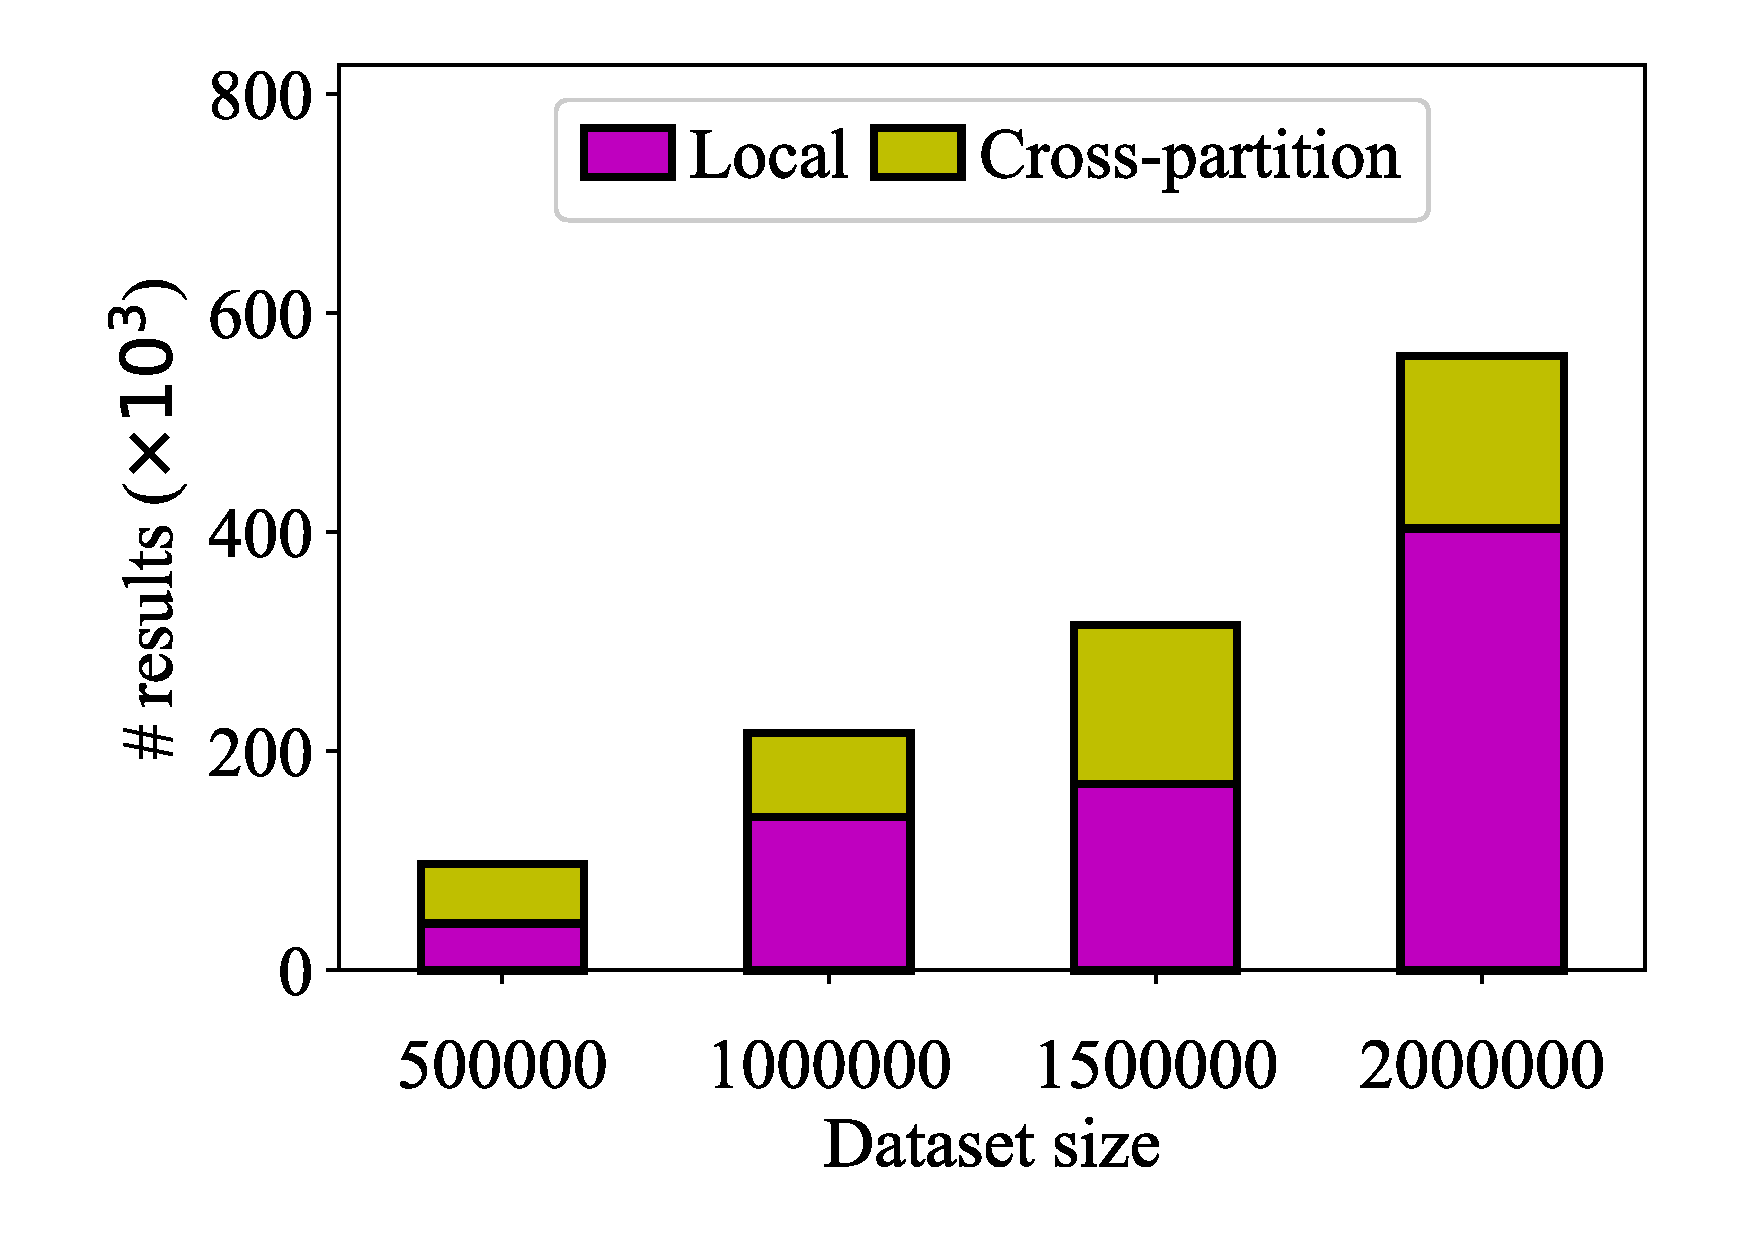
\includegraphics[trim=0.3cm 0.5cm 1.2cm 1cm, clip, width=0.32\textwidth]{figures/plots/ScalabilityResults.pdf}\label{exp:ScalabilityResults}}
 \caption{Scalability of the {\em distributed} methods.}
 \label{exp:scalability}
\end{figure*}

 \begin{figure*}[!t]
 \centering
 \subfloat[Query response time]{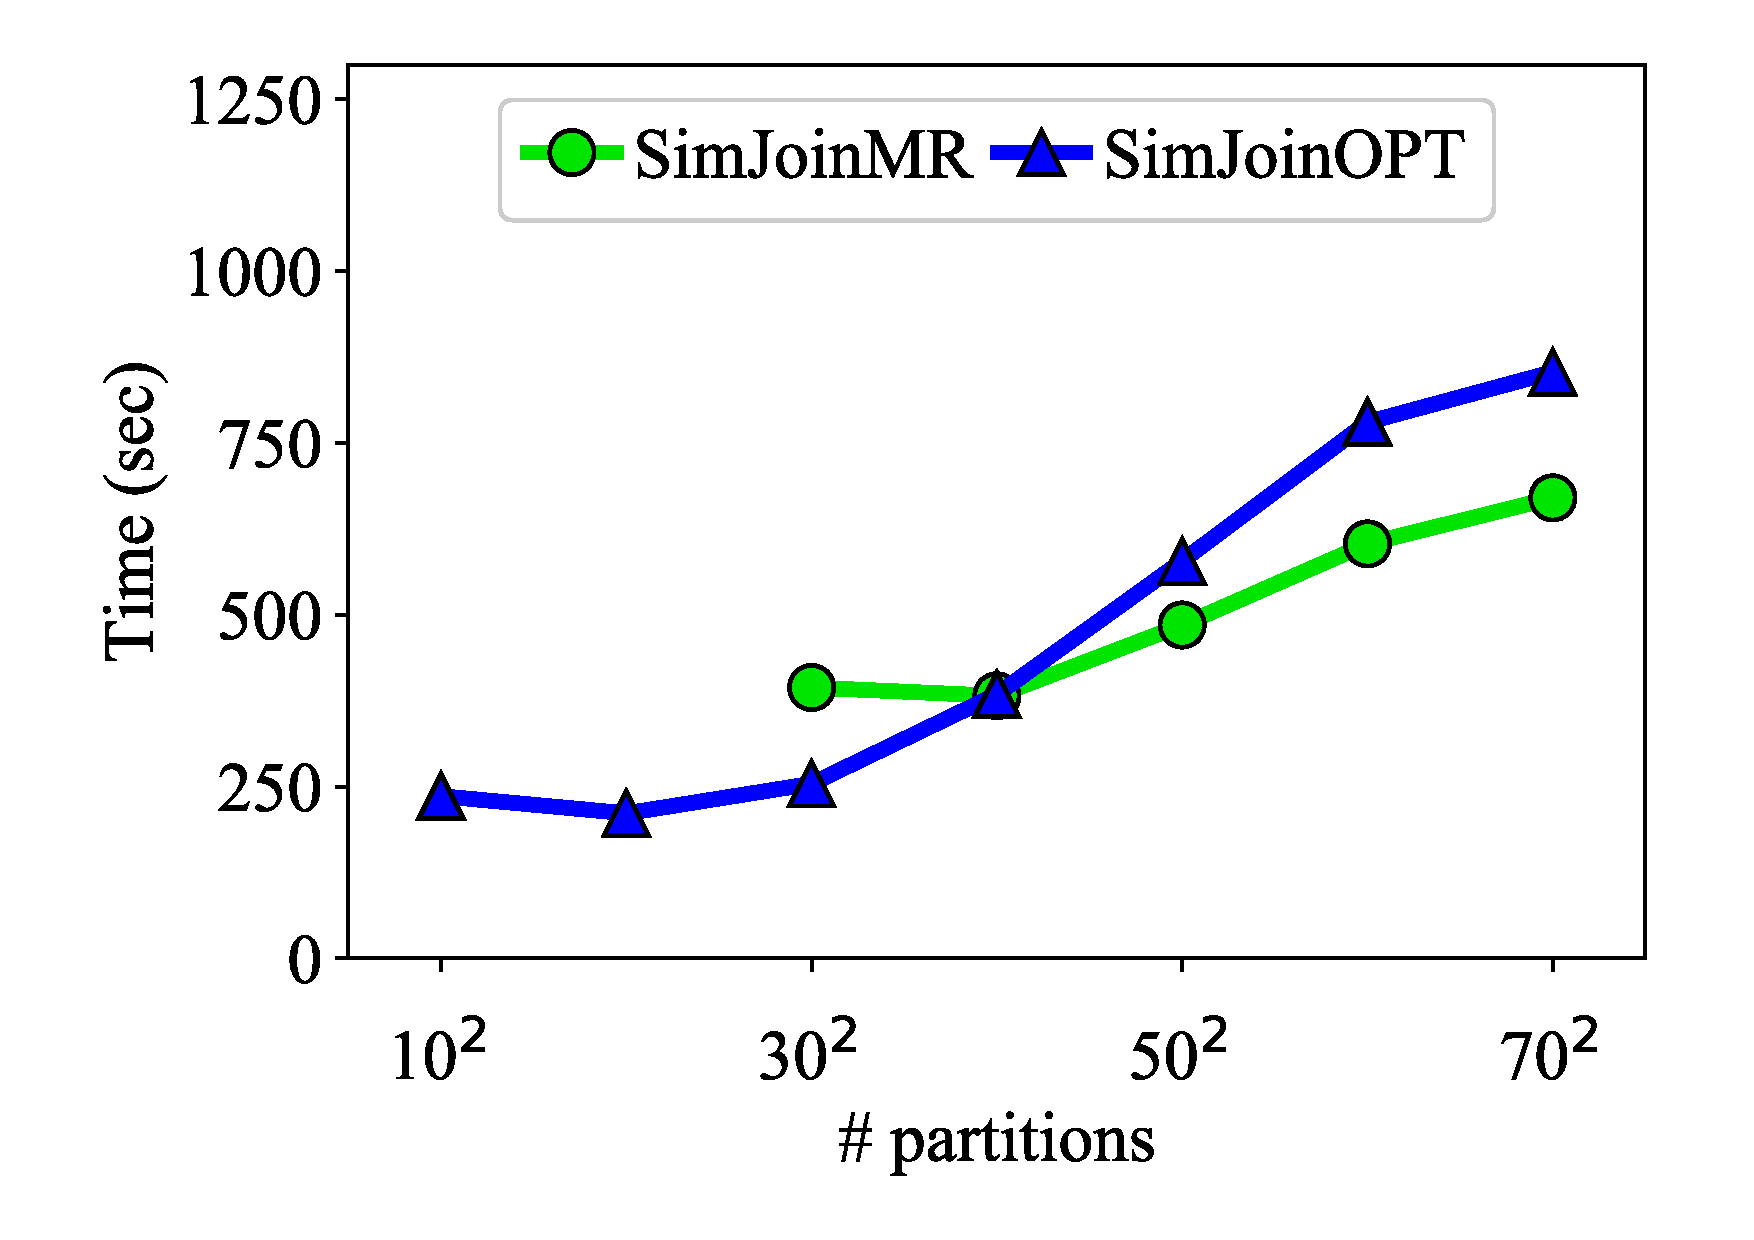
\includegraphics[trim=0.5cm 0.5cm 1cm 1cm, clip, width=0.32\textwidth]{figures/plots/Partitioning.pdf}\label{exp:Partitioning}}
 \subfloat[Geolocated time series shuffled]{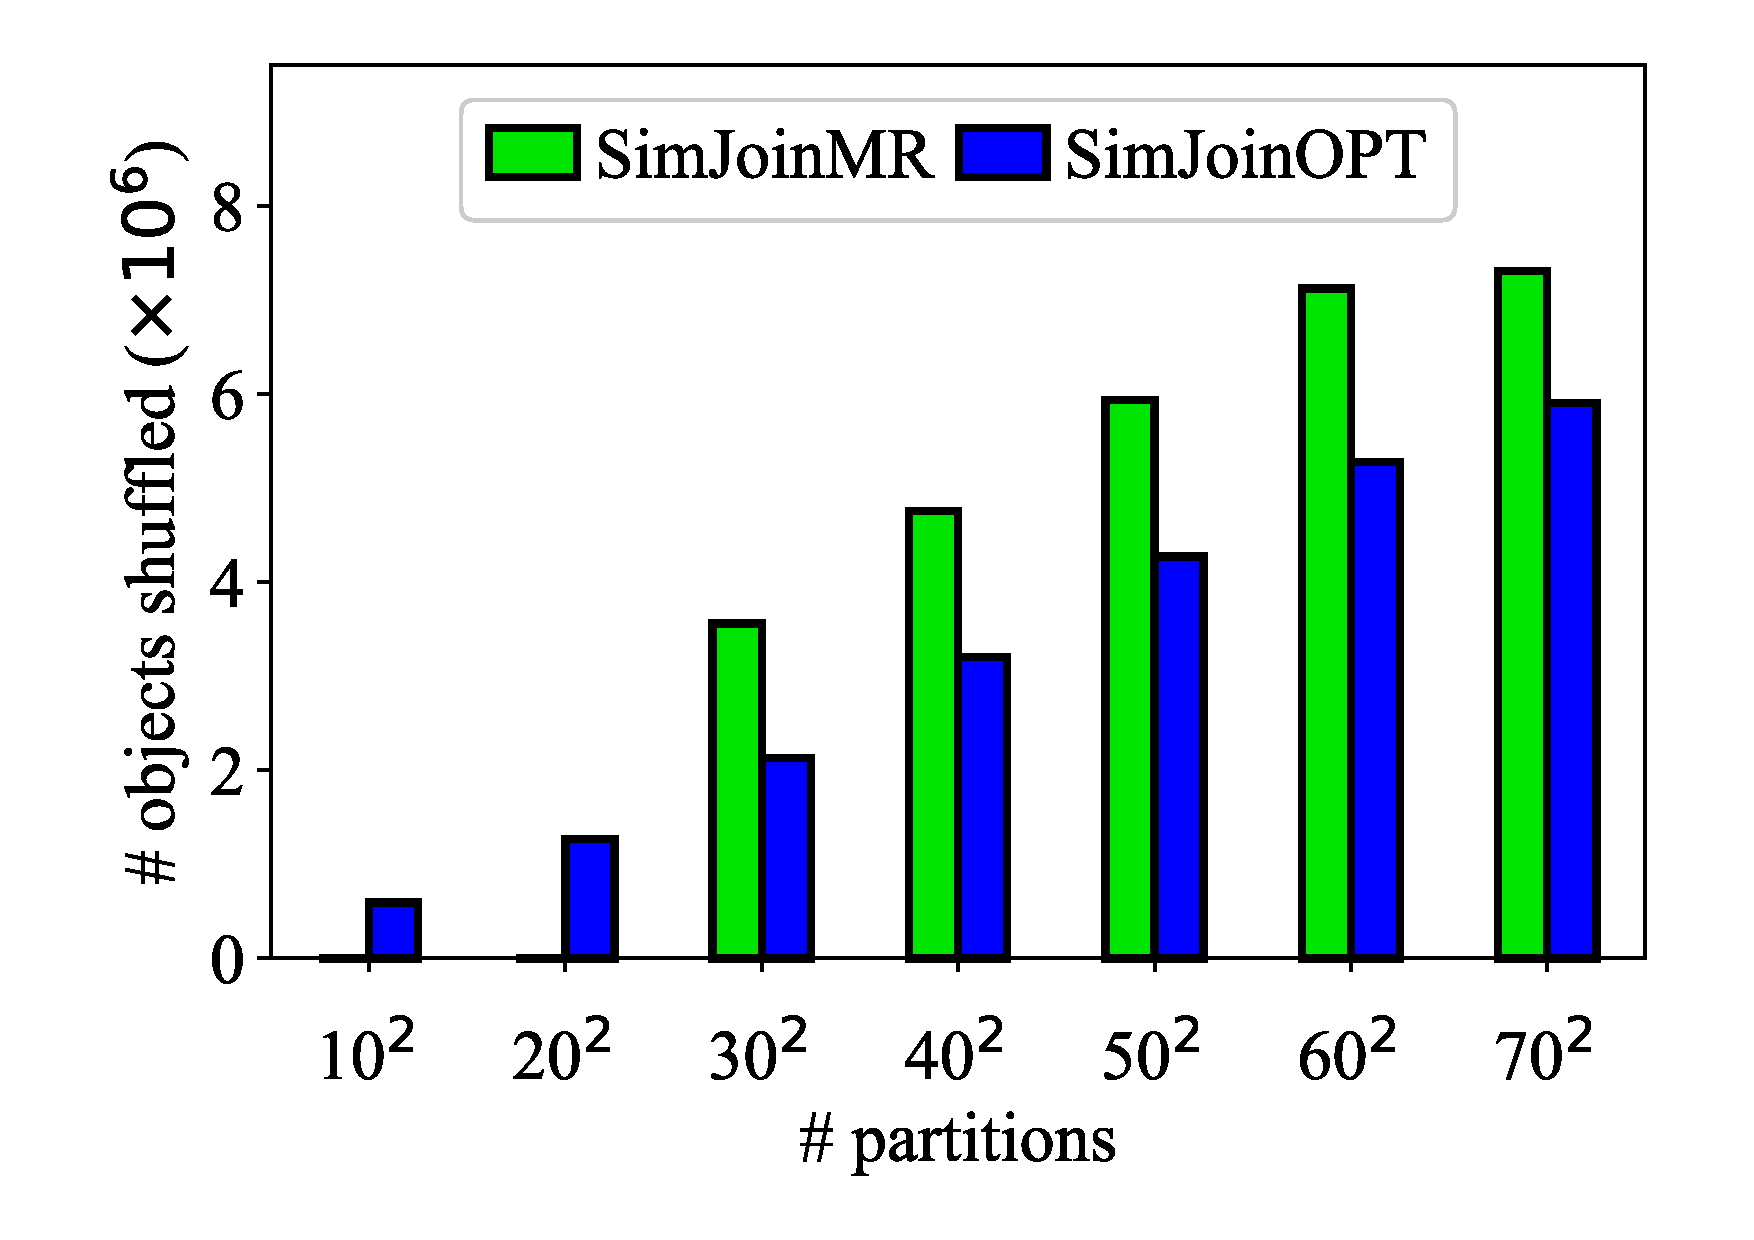
\includegraphics[trim=0.5cm 0.5cm 1cm 1cm, clip, width=0.32\textwidth]{figures/plots/PartitioningCommunication.pdf}\label{exp:PartitioningCommunication}}
 \subfloat[Number of query results per phase]{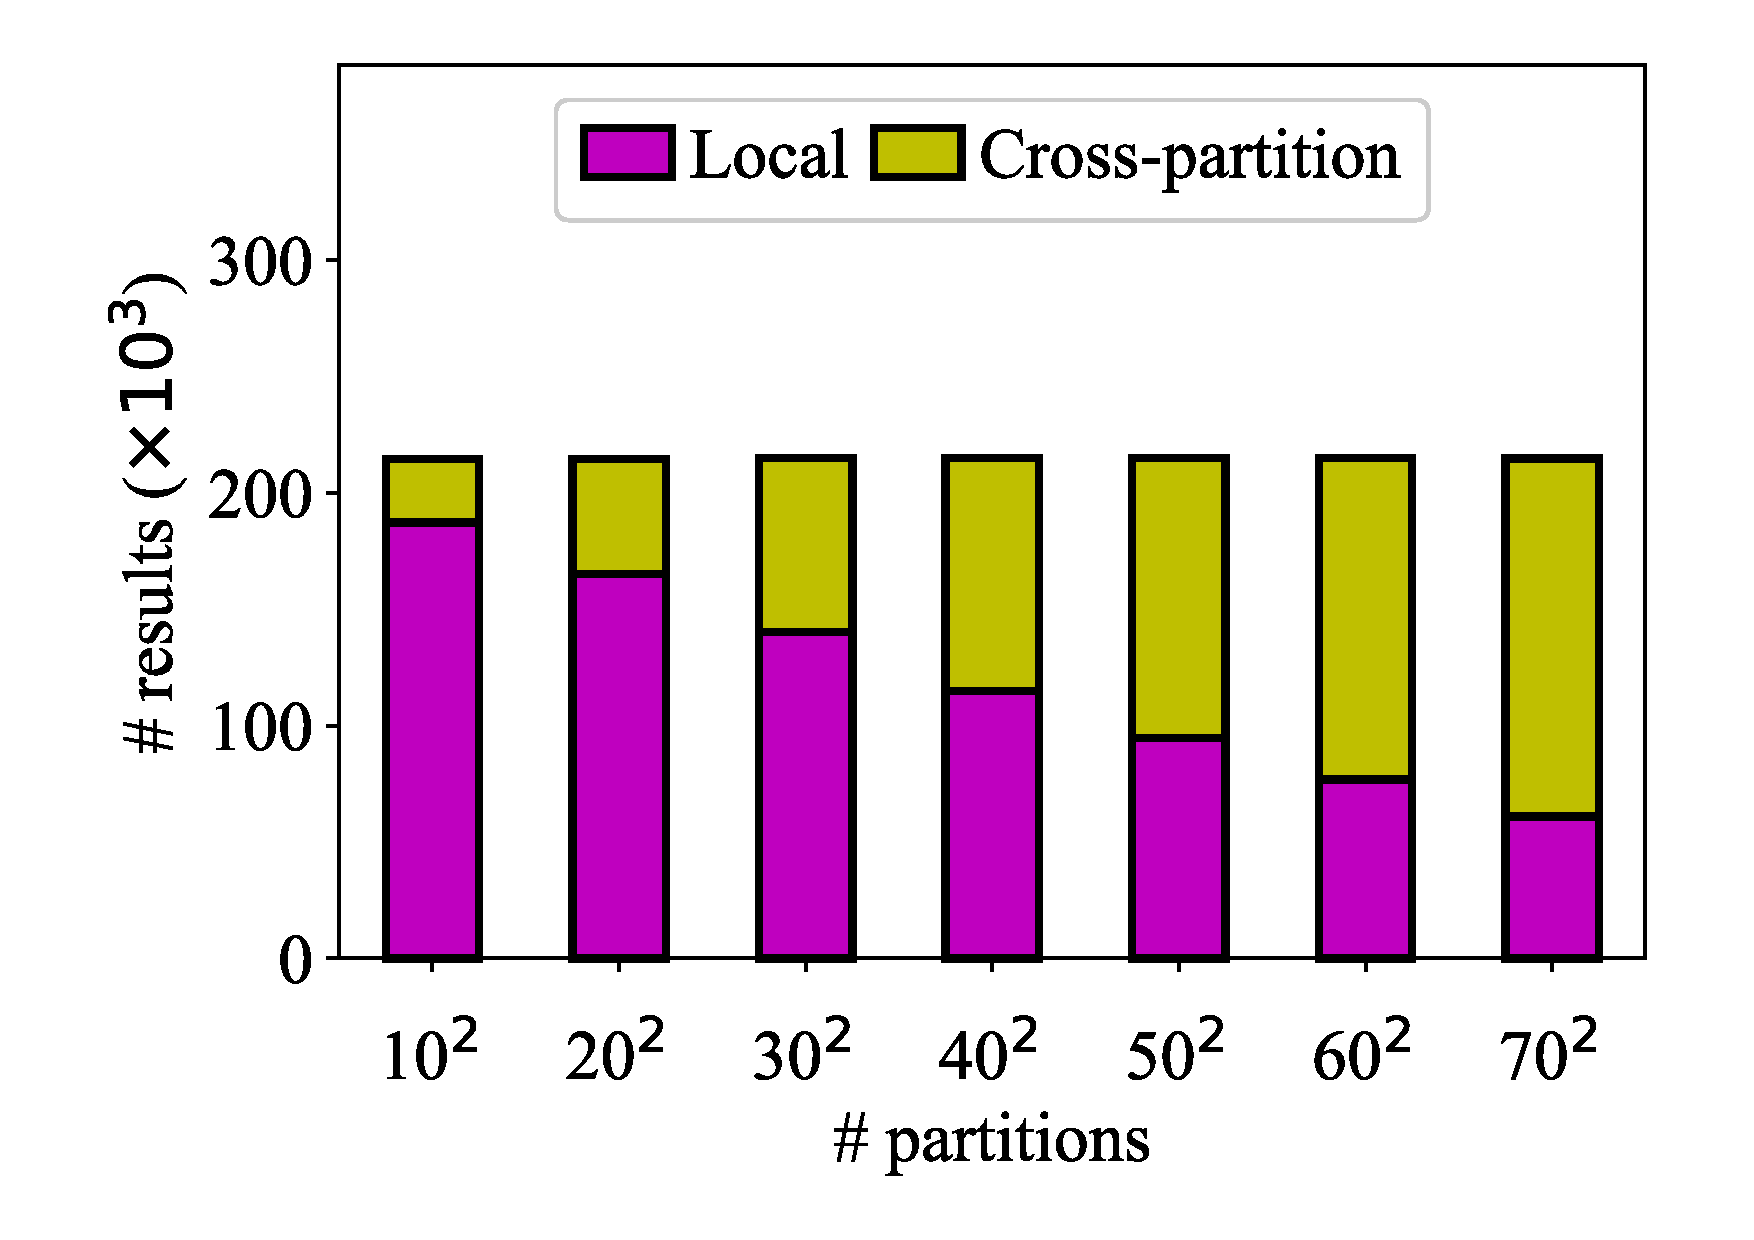
\includegraphics[trim=0.3cm 0.5cm 1.2cm 1cm, clip, width=0.32\textwidth]{figures/plots/PartitioningResults.pdf}\label{exp:PartitioningResults}}
 \caption{Effect of partitioning on the performance of {\em distributed} methods.}
 \label{exp:partitioning}
\end{figure*}



\subsubsubsection{Centralized Methods}
\label{subsec:centralized_results}


%Figure \ref{exp:centralized} depicts performance for different parameter values and dataset sizes. In these tests, the \isax-based algorithm performs significantly worse than the rest, mostly because each node comparison involves reconversion of the \isax symbols to the Euclidean space \cite{shieh2008kdd} and consequently, calculation of Euclidean distances over long sequences (up to 168 values in this data). Quite expectedly, \btsr is superior in all cases, as it is capable to prune both in the time series and spatial domains. As shown in Figure \ref{exp:EpsSPCentralized}, \btsr and \rtree-based methods perform similarly for smaller $\epsilon_{sp}$ values, as fewer candidates are found and need refinement in the time series domain. However, as distance radius $\epsilon_{sp}$ gets more relaxed, \rtree search worsens significantly, while \btsr still copes well due to its hybrid pruning ability. Of course, \isax-based search is immune to different values of $\epsilon_{sp}$, as filtering with spatial distance is only involved at refinement. With varying $\epsilon_{ts}$ values (Figure \ref{exp:EpsTSCentralized}), \btsr and \rtree approaches have practically no fluctuations in performance, as $\epsilon_{sp}$ is fixed and refinement of candidates involves a similar cost in the time series domain. But, using \isax indexing is faster for lower $\epsilon_{ts}$ values and performance slowly degrades for larger $\epsilon_{ts}$, as more candidates become eligible. In terms of scalability (Figure \ref{exp:ScalabilityCentralized}), all algorithms are almost equally fast over small datasets. But, as dataset sizes grow, the \btsr approach scales better than the rest thanks to its hybrid pruning, although the number of matching pairs escalates. Indicatively, for 100K input data, we get 2K qualifying pairs; in the 500K dataset, we get 40K results. For input data sizes larger than 500K, all centralized methods fail to finish execution, issuing an out-of-memory error. This manifests the necessity of distributed processing schemes for similarity joins over larger datasets.

Figure \ref{exp:centralized} depicts performance for different parameter values and dataset sizes. The \isax-based algorithm performs significantly worse than the rest, mostly because each node comparison involves reconversion of the \isax symbols to the Euclidean space \cite{shieh2008kdd} and consequently, calculation of Euclidean distances over long sequences (up to 168 values in this data). \btsr is superior in all cases, as it is able to prune in both time series and spatial domains. As shown in Figure \ref{exp:EpsSPCentralized}, \btsr and \rtree-based methods perform similarly for smaller $\epsilon_{sp}$ values, as fewer candidates are found and need refinement in the time series domain. However, as the distance radius $\epsilon_{sp}$ is relaxed, \rtree search worsens significantly, while \btsr still copes well due to its hybrid pruning ability. \isax-based search is immune to different values of $\epsilon_{sp}$, as filtering with spatial distance is only involved at refinement. With varying $\epsilon_{ts}$ values (Figure \ref{exp:EpsTSCentralized}), \btsr and \rtree approaches have no fluctuations in performance, as $\epsilon_{sp}$ is fixed and refinement of candidates involves a similar cost in the time series domain. However, using \isax indexing is faster for lower $\epsilon_{ts}$ values and performance slowly degrades for larger $\epsilon_{ts}$, as more candidates become eligible. In terms of scalability (Figure \ref{exp:ScalabilityCentralized}), all algorithms are almost equally fast over small datasets. But, as dataset sizes grow, the \btsr approach scales better thanks to its hybrid pruning, although the number of matching pairs escalates. Indicatively, for 100K input data, we get 2K qualifying pairs; in the 500K dataset, we get 40K results. For input data sizes larger than 500K, all centralized methods fail to finish execution, issuing an out-of-memory error. This manifests the necessity of distributed processing schemes for similarity joins over larger datasets.



\subsubsubsection{Distributed Methods}
\label{subsec:distributed_results}


%First, we compare method \base (using R-trees for local indexing) with its \opt variant (employing {\btsr}s) for varying $\epsilon_{sp}$ values. It is apparent from Figure \ref{exp:EpsSPDist} that query response times for the \base method are increasing, since the underlying {\rtree}s fare worse for larger distance radii (also confirmed in the centralized tests in Figure \ref{exp:EpsSPCentralized}). With larger $\epsilon_{sp}$ values, more raw data has to be shuffled between workers during the cross-partition checks, as the size of bands and boxes involved gets bigger and covers more candidate objects. Concerning exactly this shuffling overhead, Figure~\ref{exp:EpsSPDistCommunication} reveals that this is indeed much lower in the \opt variant, which explains its processing cost advantage. Finally, Figure \ref{exp:EpsSPDistResults} illustrates the number of results produced from the two stages; first locally in each partition, and then after cross-partition checks in bands and boxes. As distance constraint $\epsilon_{sp}$ gets more relaxed, more pairs qualify as answers. For smaller $\epsilon_{sp}$, the majority of results come locally from each partition. But as $\epsilon_{sp}$ is relaxed, many more pairs are found in neighboring partitions during the cross-partition checks, as bands and corner-wise boxes also become larger and increase their share in qualifying results much more.

First, we compare \base (using R-trees for local indexing) with its \opt variant (employing {\btsr}s) for varying $\epsilon_{sp}$ values. It is apparent from Figure \ref{exp:EpsSPDist} that query response times for the \base method are increasing, since the underlying {\rtree}s fare worse for larger distance radii. With larger $\epsilon_{sp}$ values, more raw data has to be shuffled between workers during the cross-partition checks, as the size of bands and boxes involved gets bigger and covers more candidate objects. Concerning exactly this shuffling overhead, Figure~\ref{exp:EpsSPDistCommunication} reveals that this is indeed lower in the \opt variant, which explains its processing cost advantage. Finally, Figure \ref{exp:EpsSPDistResults} illustrates the number of results produced from the two stages; first locally in each partition, and then after cross-partition checks in bands and boxes. As distance constraint $\epsilon_{sp}$ gets more relaxed, more pairs qualify as answers. For smaller $\epsilon_{sp}$, the majority of results come locally from each partition. But as $\epsilon_{sp}$ is relaxed, many more pairs are found in neighboring partitions, as bands and boxes also become larger and increase their share in qualifying results much more.


With regard to increasing $\epsilon_{ts}$ values, observe in Figure \ref{exp:EpsTSDist} that method \base is consistently worse than \opt, basically due to the different pruning power of their respective indices. The former relies on R-trees, which have no effect with varying $\epsilon_{ts}$; in contrast, {\btsr}s employed by \opt can effectively filter candidates also in the time series domain. With a more relaxed $\epsilon_{ts}$, more results qualify, hence the linear increase in processing cost. Regarding the data shuffling overhead, this is practically stable for each method irrespective of the $\epsilon_{ts}$ constraint (Figure \ref{exp:EpsTSDistCommunication}). In \base, selection of objects that should be transmitted is solely based on their spatial containment in the respective bands and corner-wise boxes. But \opt spares transferring many irrelevant objects, as it also uses filtering with $\epsilon_{ts}$; the amount of dispatched objects is only slightly increasing with $\epsilon_{ts}$. Regarding the number of generated results, Figure \ref{exp:EpsTSDistResults} reveals a rather steep increase for small variations of $\epsilon_{ts}$, which indicates that most time series are clustered within a small range of $\epsilon_{ts}$ deviations. As original data concern water consumption, this explains such highly correlated behavior, especially among neighboring households; of course, this pattern is replicated in the synthetic data as well. The percentage of results from cross-partition checks in each full answer is similar across various $\epsilon_{ts}$ values, as distance $\epsilon_{sp}$ is fixed and so are the respective bands and boxes involved in this phase.


Figure \ref{exp:scalability} concerns scalability of the distributed methods with increasing dataset sizes. For smaller datasets, both methods are competitive, but response times for \base escalate with larger sizes. With 2 million objects as input, this method did not finish, as it required traversal of too many paths in its underlying R-trees per partition, exceeding the capabilities of the workers. Regarding communication (Figure \ref{sexp:ScalabilityCommunication}), \base requires shuffling of more raw data, especially for input size of 1.5 million. In contrast, \opt maintains lower communication overhead, as it uses light-weight indices to guide data shuffling. Figure \ref{exp:ScalabilityResults} indicates that the number of results is growing according to the input size, as the spatial density also increases with larger synthetic datasets that still cover  the same area (Alicante).



Last but not least, we conducted tests concerning partitioning, i.e., varying the grid granularity and distributing input data accordingly. As shown in Figure \ref{exp:Partitioning}, \base was not able to conclude its evaluation over coarser spatial subdivisions, as each resulting partition can hardly cope with the larger subsets of data held locally. For $30 \times 30$ partitions, \opt performs better thanks to  the superiority of \btsr in pruning. But \base overtakes \opt when allowing finer partitioning ($40 \times 40$ partitions or more), as the \rtree overhead diminishes. Each such index has to deal with smaller subsets, although it incurs higher communication overhead compared to \opt (Figure \ref{exp:PartitioningCommunication}). Indeed, having more partitions forces \opt to search for joins pairwise in many more bands and boxes, while also building the respective intermediate indices. So, such optimization really compensates with a coarser partitioning, achieving its best performance with a $20 \times 20$ grid as depicted in Figure \ref{exp:Partitioning}. Finally, Figure \ref{exp:PartitioningResults} indicates that the majority of resulting pairs are derived locally under a coarser partitioning. However, this is reversed with finer partitioning, as the size of blocks (bands and boxes) during the cross-partition checks cover much more area per cell, hence many more qualifying pairs are found while searching across neighboring partitions.

%\mnote{If {\em Baseline} is the one using R-tree index, does it makes sense to run experiments also for its \btsr counterpart (i.e., without the optimization of light-joins)?}